\chapter{約書亞記}
\section{攻打迦南 1-12 }
\subsection{立约书亚为领袖 1 }
\subsubsection{上帝給約書亞的应许及勉励 1:1-9 }
\begin{table}[H]
\begin{tabular}{ p{10.4cm}|p{6.8cm}} \toprule
耶和華給約書亞的应许&給約書亞的勉励        \\\hline
耶和華的僕人摩西死了以後，耶和華曉諭摩西的幫手，嫩的兒子約書亞，說：「我的僕人摩西死了，現在你要起來，和眾百姓過這約旦河，往我所要賜給以色列人的地去。凡你們腳掌所踏之地，我都照著我所應許摩西的話賜給你們了。從曠野和這黎巴嫩，直到伯拉大河，赫人的全地，又到大海日落之處，都要做你們的境界。你平生的日子，必無一人能在你面前站立得住。我怎樣與摩西同在，也必照樣與你同在。我必不撇下你，也不丟棄你。你當剛強壯膽，因為你必使這百姓承受那地為業，就是我向他們列祖起誓應許賜給他們的地。 &只要剛強，大大壯膽，謹守遵行我僕人摩西所吩咐你的一切律法，不可偏離左右，使你無論往哪裡去，都可以順利。這律法書不可離開你的口，總要晝夜思想，好使你謹守遵行這書上所寫的一切話。如此，你的道路就可以亨通，凡事順利。我豈沒有吩咐你嗎？你當剛強壯膽！不要懼怕，也不要驚惶，因為你無論往哪裡去，耶和華你的神必與你同在。」\\\hline
\bottomrule
\end{tabular}
\caption{給約書亞的应许及勉励}
\label{table:sci}
\end{table}


\subsubsection{约书亚对百姓的要求 1:10-11 }
於是，約書亞吩咐百姓的官長說：「你們要走遍營中，吩咐百姓說：『當預備食物，因為三日之內你們要過這約旦河，進去得耶和華你們神賜你們為業之地。』

\subsubsection{约书亚吩咐河东两个半支派 1:12-18 }
\begin{table}[H]
\begin{tabular}{ p{10.8cm}|p{6.5cm}} \toprule
耶和華指給摩西看&禁止摩西過到那应许之地          \\\hline
約書亞對魯本人、迦得人和瑪拿西半支派的人說：「你們要追念耶和華的僕人摩西所吩咐你們的話說：耶和華你們的神使你們得享平安，也必將這地賜給你們。你們的妻子孩子和牲畜都可以留在約旦河東摩西所給你們的地。但你們中間一切大能的勇士都要帶著兵器在你們的弟兄前面過去幫助他們，等到耶和華使你們的弟兄像你們一樣得享平安，並且得著耶和華你們神所賜他們為業之地，那時才可以回你們所得之地承受為業，就是耶和華的僕人摩西在約旦河東向日出之地所給你們的。」&他們回答約書亞說：「你所吩咐我們行的，我們都必行；你所差遣我們去的，我們都必去。我們從前在一切事上怎樣聽從摩西，現在也必照樣聽從你。唯願耶和華你的神與你同在，像與摩西同在一樣。無論什麼人違背你的命令，不聽從你所吩咐他的一切話，就必治死他。你只要剛強壯膽。」\\\hline
\bottomrule
\end{tabular}
\caption{约书亚对与河东两个半支派的对话}
\label{table:sci}
\end{table}



\subsection{攻打耶利哥 2-6 }

\subsubsection{喇合隐藏两个探子 2:1-7}
當下，嫩的兒子約書亞從什亭暗暗打發兩個人做探子，吩咐說：「你們去窺探那地和耶利哥。」於是二人去了，來到一個妓女名叫喇合的家裡，就在那裡躺臥。有人告訴耶利哥王說：「今夜有以色列人來到這裡窺探此地。」耶利哥王打發人去見喇合說：「那來到你這裡，進了你家的人要交出來，因為他們來窺探全地。」女人將二人隱藏，就回答說：「那人果然到我這裡來，他們是哪裡來的我卻不知道。天黑要關城門的時候他們出去了，往哪裡去我卻不知道。你們快快地去追趕，就必追上。」（先是女人領二人上了房頂，將他們藏在那裡所擺的麻秸中。）那些人就往約旦河的渡口追趕他們去了。追趕他們的人一出去，城門就關了。

\subsubsection{喇合求探子救全家 2:8-13}
二人還沒有躺臥，女人就上房頂，到他們那裡，對他們說：「我知道耶和華已經把這地賜給你們，並且因你們的緣故我們都驚慌了。這地的一切居民在你們面前心都消化了。因為我們聽見你們出埃及的時候，耶和華怎樣在你們前面使紅海的水乾了，並且你們怎樣待約旦河東的兩個亞摩利王西宏和噩，將他們盡行毀滅。我們一聽見這些事，心就消化了。因你們的緣故，並無一人有膽氣，耶和華你們的神本是上天下地的神。現在我既是恩待你們，求你們指著耶和華向我起誓，也要恩待我父家，並給我一個實在的證據，要救活我的父母、弟兄、姐妹和一切屬他們的，拯救我們性命不死。」 

\subsubsection{喇合全家蒙拯救的条件 2:14-21}
二人對她說：「你若不洩漏我們這件事，我們情願替你們死。耶和華將這地賜給我們的時候，我們必以慈愛、誠實待你。」

 於是女人用繩子將二人從窗戶裡縋下去，因她的房子是在城牆邊上，她也住在城牆上。她對他們說：「你們且往山上去，恐怕追趕的人碰見你們。要在那裡隱藏三天，等追趕的人回來，然後才可以走你們的路。」二人對她說：「你要這樣行，不然，你叫我們所起的誓就與我們無干了。我們來到這地的時候，你要把這條朱紅線繩繫在縋我們下去的窗戶上，並要使你的父母、弟兄和你父的全家都聚集在你家中。凡出了你家門往街上去的，他的罪（血）必歸到自己的頭上，與我們無干了。凡在你家裡的，若有人下手害他，流他血的罪就歸到我們的頭上。你若洩漏我們這件事，你叫我們所起的誓就與我們無干了。」 女人說：「照你們的話行吧。」於是打發他們去了，又把朱紅線繩繫在窗戶上。


\subsubsection{两个探子返回营地 2:22-24}
二人到山上，在那裡住了三天，等著追趕的人回去了。追趕的人一路找他們，卻找不著。 23 二人就下山回來，過了河，到嫩的兒子約書亞那裡，向他述說所遭遇的一切事。 24 又對約書亞說：「耶和華果然將那全地交在我們手中，那地的一切居民在我們面前心都消化了。」

\subsubsection{約書亞率百姓过约旦河 3:1-6}
約書亞清早起來，和以色列眾人都離開什亭，來到約旦河，就住在那裡，等候過河。 2 過了三天，官長走遍營中， 3 吩咐百姓說：「你們看見耶和華你們神的約櫃，又見祭司利未人抬著，就要離開所住的地方，跟著約櫃去。 4 只是你們和約櫃相離要量二千肘，不可與約櫃相近，使你們知道所當走的路，因為這條路你們向來沒有走過。」 5 約書亞吩咐百姓說：「你們要自潔，因為明天耶和華必在你們中間行奇事。」 6 約書亞又吩咐祭司說：「你們抬起約櫃，在百姓前頭過去。」於是他們抬起約櫃，在百姓前頭走。

\subsubsection{耶和華吩咐約書亞 3:7-13}
耶和華對約書亞說：「從今日起，我必使你在以色列眾人眼前尊大，使他們知道我怎樣與摩西同在，也必照樣與你同在。 8 你要吩咐抬約櫃的祭司說：『你們到了約旦河的水邊上，就要在約旦河水裡站住。』」 9 約書亞對以色列人說：「你們近前來，聽耶和華你們神的話。」 10  11 約書亞說：「看哪，普天下主的約櫃必在你們前頭過去，到約旦河裡，因此你們就知道在你們中間有永生神，並且他必在你們面前趕出迦南人、赫人、希未人、比利洗人、革迦撒人、亞摩利人、耶布斯人。 12 你們現在要從以色列支派中揀選十二個人，每支派一人。 13 等到抬普天下主耶和華約櫃的祭司把腳站在約旦河水裡，約旦河的水，就是從上往下流的水，必然斷絕，立起成壘。」

\subsubsection{眾人從乾地過了約旦河 3:14-17}
百姓離開帳篷要過約旦河的時候，抬約櫃的祭司乃在百姓的前頭。 15 他們到了約旦河，腳一入水（原來約旦河水在收割的日子漲過兩岸）， 16 那從上往下流的水，便在極遠之地，撒拉但旁的亞當城那裡停住，立起成壘。那往亞拉巴的海，就是鹽海，下流的水全然斷絕。於是百姓在耶利哥的對面過去了。 17 抬耶和華約櫃的祭司在約旦河中的乾地上站定，以色列眾人都從乾地上過去，直到國民盡都過了約旦河。

\subsubsection{取約旦河石立在吉甲為紀念 4:1-8}
 \begin{figure}[H]
    %\centering
	 \begin{center}%[圖2：利未各支派職分及位置]
	 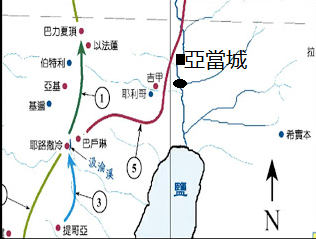
\includegraphics[width=3in]{BLiShiFigs/jordan}
	 \caption{以色列人過約旦河的位置}
	 \label{fig:1} 
	 \end{center}
	 \end{figure}
國民盡都過了約旦河，耶和華就對約書亞說： 2 「你從民中要揀選十二個人，每支派一人， 3 吩咐他們說：『你們從這裡，從約旦河中，祭司腳站定的地方，取十二塊石頭帶過去，放在你們今夜要住宿的地方。』」 4 於是，約書亞將他從以色列人中所預備的那十二個人，每支派一人，都召了來， 5 對他們說：「你們下約旦河中，過到耶和華你們神的約櫃前頭，按著以色列人十二支派的數目，每人取一塊石頭扛在肩上。 6 這些石頭在你們中間可以作為證據。日後，你們的子孫問你們說：『這些石頭是什麼意思？』 7 你們就對他們說：『這是因為約旦河的水在耶和華的約櫃前斷絕。約櫃過約旦河的時候，約旦河的水就斷絕了。這些石頭要做以色列人永遠的紀念。』」

以色列人就照約書亞所吩咐的，按著以色列人支派的數目，從約旦河中取了十二塊石頭，都遵耶和華所吩咐約書亞的行了。他們把石頭帶過去，到他們所住宿的地方，就放在那裡。

\subsubsection{取約旦河石立在祭司腳站立的地方 4:9}
約書亞另把十二塊石頭立在約旦河中，在抬約櫃的祭司腳站立的地方，直到今日那石頭還在那裡。

\subsubsection{眾百姓和两个半支派的四萬人都過了河 4:10-13}
抬約櫃的祭司站在約旦河中，等到耶和華曉諭約書亞吩咐百姓的事辦完了，是照摩西所吩咐約書亞的一切話。於是百姓急速過去了。 11 眾百姓盡都過了河，耶和華的約櫃和祭司就在百姓面前過去。 12 魯本人、迦得人、瑪拿西半支派的人都照摩西所吩咐他們的，帶著兵器在以色列人前頭過去。 13 約有四萬人都準備打仗，在耶和華面前過去，到耶利哥的平原，等候上陣。

\subsubsection{約但河的水仍舊漲過兩岸 4:14-18}
當那日，耶和華使約書亞在以色列眾人眼前尊大。在他平生的日子，百姓敬畏他，像從前敬畏摩西一樣。

15 耶和華曉諭約書亞說： 16 「你吩咐抬法櫃的祭司從約旦河裡上來。」 17 約書亞就吩咐祭司說：「你們從約旦河裡上來。」 18 抬耶和華約櫃的祭司從約旦河裡上來，腳掌剛落旱地，約旦河的水就流到原處，仍舊漲過兩岸。
祭司從約但河裡上來，腳掌剛落旱地，約但河的水仍舊漲過兩岸

\subsubsection{約書亞在吉甲重申十二塊石頭的意思 4:19-24}
正月初十日，百姓從約旦河裡上來，就在吉甲，在耶利哥的東邊安營。 20 他們從約旦河中取來的那十二塊石頭，約書亞就立在吉甲， 21 對以色列人說：「日後你們的子孫問他們的父親說：『這些石頭是什麼意思？』 22 你們就告訴他們說：『以色列人曾走乾地過這約旦河。 23 因為耶和華你們的神在你們前面使約旦河的水乾了，等著你們過來，就如耶和華你們的神從前在我們前面使紅海乾了，等著我們過來一樣。 24 要使地上萬民都知道耶和華的手大有能力，也要使你們永遠敬畏耶和華你們的神。』」
    
\begin{table}[H]
\begin{threeparttable}
\begin{tabular}{@{}p{0.18\textwidth}*{2}{L{\dimexpr0.8\linewidth-10\tabcolsep\relax}}@{}}
\toprule
發命令的人 & 命令\\\hline
官長吩咐百姓 & 你們看見耶和華─你們神的約櫃，又見祭司利未人擡著，就要離開所住的地方，跟著約櫃去。只是你們和約櫃相離要量二千肘，不可與約櫃相近，使你們知道所當走的路，因為這條路你們向來沒有走過。 \\\hline
約書亞吩咐百姓說&你們要自潔，因為明天耶和華必在你們中間行奇事。\\\hline
約書亞又吩咐祭司說 & 你們擡起約櫃，在百姓前頭過去。於是他們擡起約櫃，在百姓前頭走。 \\\hline
耶和華對約書亞說 &從今日起，我必使你在以色列眾人眼前尊大，使他們知道我怎樣與摩西同在，也必照樣與你同在。你要吩咐擡約櫃的祭司說：你們到了約但河的水邊上，就要在約但河水裡站住。\\\hline
約書亞對以色列人說& 你們近前來，聽耶和華─你們神的話。看哪，普天下主的約櫃必在你們前頭過去，到約但河裡，因此你們就知道在你們中間有永生神；並且他必在你們面前趕出迦南人、赫人、希未人、比利洗人、革迦撒人、亞摩利人、耶布斯人。你們現在要從以色列支派中揀選十二個人，每支派一人，等到擡普天下主耶和華約櫃的祭司把腳站在約但河水裡，約但河的水，就是從上往下流的水，必然斷絕，立起成壘。\tabularnewline
\hline
\bottomrule
\end{tabular}
%\end{tabularx}
\caption{預備過約旦河}
\end{threeparttable}
\end{table} 


\subsubsection{迦南人聞而膽消 5:1}
約旦河西亞摩利人的諸王和靠海迦南人的諸王，聽見耶和華在以色列人前面使約旦河的水乾了，等到我們過去，他們的心因以色列人的緣故就消化了，不再有膽氣。

\subsubsection{在吉甲行割礼 5:2-9}
\begin{wraptable}{r}{10cm}
\centering
\begin{tabular}{|c|c|}
\hline
\hline
日期                   & 事件   \\\hline
正月10日               & 過約但河    \\\hline
正月10日- 13日 & 割禮\\\hline
正月十四日             & 耶利哥平原守逾越節   \\\hline
逾越節次日           & 吃那地出產（無酵餅和烘的穀）\\\hline
正月16日             & 嗎哪止住　\\\hline
\end{tabular}
\caption{過約旦河後的經歷}
\end{wraptable}
那時，耶和華吩咐約書亞說：「你製造火石刀，第二次給以色列人行割禮。」 3 約書亞就製造了火石刀，在除皮山那裡給以色列人行割禮。 4 約書亞行割禮的緣故，是因為從埃及出來的眾民，就是一切能打仗的男丁，出了埃及以後都死在曠野的路上， 5 因為出來的眾民都受過割禮，唯獨出埃及以後，在曠野的路上所生的眾民都沒有受過割禮。 6 以色列人在曠野走了四十年，等到國民，就是出埃及的兵丁，都消滅了，因為他們沒有聽從耶和華的話。耶和華曾向他們起誓，必不容他們看見耶和華向他們列祖起誓應許賜給我們的地，就是流奶與蜜之地。 7 他們的子孫，就是耶和華所興起來接續他們的，都沒有受過割禮。因為在路上沒有給他們行割禮，約書亞這才給他們行了。 8 國民都受完了割禮，就住在營中自己的地方，等到痊癒了。 9 耶和華對約書亞說：「我今日將埃及的羞辱從你們身上滾去了。」因此那地方名叫吉甲(滾)，直到今日。

\subsubsection{守逾越節 5:10-11}
以色列人在吉甲安營。正月十四日晚上，在耶利哥的平原守逾越節。逾越節的次日，他們就吃了那地的出產，正當那日吃無酵餅和烘的穀。

\subsubsection{嗎哪止降 5:12}
他們吃了那地的出產，第二日嗎哪就止住了，以色列人也不再有嗎哪了。那一年，他們卻吃迦南地的出產。

\subsubsection{約書亞見耶和華軍帥 5:13-15}
\begin{table}[H]
\begin{tabular}{ p{9.cm}|p{8.cm}} \toprule
\toprule
約書亞 &  耶和华军队的元帅 \\\hline
約書亞靠近耶利哥的時候，舉目觀看， &不料，有一個人手裡有拔出來的刀，對面站立。\tabularnewline
約書亞到他那裡，問他說：「你是幫助我們呢，是幫助我們敵人呢？」 &他回答說：「不是的，我來是要做耶和華軍隊的元帥。」 \tabularnewline
約書亞就俯伏在地下拜，說：「我主有什麼話吩咐僕人？」  &耶和華軍隊的元帥對約書亞說：「把你腳上的鞋脫下來，因為你所站的地方是聖的。」\tabularnewline
約書亞就照著行了。& \tabularnewline
\hline\bottomrule
\end{tabular}
\caption{約書亞見耶和華軍帥}
\end{table} 

\subsubsection{耶和華曉諭約書亞攻城方法 6:1-5}
\begin{table}{r}{10cm}
\centering
\begin{tabular}{|c|c|}
\hline
\hline
日期   & 攻城過程   \\\hline
第一日 & 繞城一次，祭司吹角，百姓不可出聲    \\\hline
第二日 & 繞城一次，祭司吹角，百姓不可出聲\\\hline
第三日 & 繞城一次，祭司吹角，百姓不可出聲 \\\hline
第四日 & 繞城一次，祭司吹角，百姓不可出聲\\\hline
第五日 & 繞城一次，祭司吹角，百姓不可出聲\\\hline
第六日 & 繞城一次，祭司吹角，百姓不可出聲　\\\hline
第七日 & 繞城七次，祭司吹角，角聲拖長時，百姓吶喊　\\\hline
\end{tabular}
\caption{攻陷耶利哥}
\end{table}
耶利哥的城門因以色列人就關得嚴緊，無人出入。 2 耶和華曉諭約書亞說：「看哪，我已經把耶利哥和耶利哥的王，並大能的勇士，都交在你手中。 3 你們的一切兵丁要圍繞這城，一日圍繞一次，六日都要這樣行。 4 七個祭司要拿七個羊角走在約櫃前。到第七日，你們要繞城七次，祭司也要吹角。 5 他們吹的角聲拖長，你們聽見角聲，眾百姓要大聲呼喊，城牆就必塌陷，各人都要往前直上。」


\subsubsection{約書亞吩咐攻百姓遵守 6:6-7}
嫩的兒子約書亞召了祭司來，吩咐他們說：「你們抬起約櫃來，要有七個祭司拿七個羊角走在耶和華的約櫃前。」 7 又對百姓說：「你們前去繞城，帶兵器的要走在耶和華的約櫃前。」

\subsubsection{以色列人繞耶利哥城六日 6:8-14}
約書亞對百姓說完了話，七個祭司拿七個羊角走在耶和華面前吹角，耶和華的約櫃在他們後面跟隨。 9 帶兵器的走在吹角的祭司前面，後隊隨著約櫃行。祭司一面走一面吹。 10 約書亞吩咐百姓說：「你們不可呼喊，不可出聲，連一句話也不可出你們的口，等到我吩咐你們呼喊的日子，那時才可以呼喊。」 11 這樣，他使耶和華的約櫃繞城，把城繞了一次。眾人回到營裡，就在營裡住宿。

12 約書亞清早起來，祭司又抬起耶和華的約櫃。 13 七個祭司拿七個羊角在耶和華的約櫃前，時常行走吹角。帶兵器的在他們前面走，後隊隨著耶和華的約櫃行。祭司一面走一面吹。 14 第二日，眾人把城繞了一次，就回營裡去。六日都是這樣行。

\subsubsection{第七日約書亞吩咐百姓，城塌陷 6:15-21}
第七日清早，黎明的時候，他們起來，照樣繞城七次。唯獨這日把城繞了七次。 16 到了第七次，祭司吹角的時候，約書亞吩咐百姓說：「呼喊吧！因為耶和華已經把城交給你們了。 17 這城和其中所有的都要在耶和華面前毀滅，只有妓女喇合與她家中所有的可以存活，因為她隱藏了我們所打發的使者。 18 至於你們，務要謹慎，不可取那當滅的物，恐怕你們取了那當滅的物就連累以色列的全營，使全營受咒詛。 19 唯有金子、銀子和銅鐵的器皿，都要歸耶和華為聖，必入耶和華的庫中。」 20 於是百姓呼喊，祭司也吹角。百姓聽見角聲，便大聲呼喊，城牆就塌陷。百姓便上去進城，各人往前直上，將城奪取。 21 又將城中所有的，不拘男女老少，牛羊和驢，都用刀殺盡。

\subsubsection{喇合並她一切的親眷蒙救 6:22-25}
約書亞吩咐窺探地的兩個人說：「你們進那妓女的家，照著你們向她所起的誓，將那女人和她所有的都從那裡帶出來。」 23 當探子的兩個少年人就進去，將喇合與她的父母、弟兄和她所有的，並她一切的親眷，都帶出來，安置在以色列的營外。 24 眾人就用火將城和其中所有的焚燒了。唯有金子、銀子和銅鐵的器皿，都放在耶和華殿的庫中。 25 約書亞卻把妓女喇合與她父家，並她所有的，都救活了，因為她隱藏了約書亞所打發窺探耶利哥的使者。她就住在以色列中，直到今日。

\subsubsection{修耶利哥所受的咒詛 6:26-27}

 26 當時，約書亞叫眾人起誓說：「有興起重修這耶利哥城的人，當在耶和華面前受咒詛：他立根基的時候，必喪長子；安門的時候，必喪幼子。」 27 耶和華與約書亞同在，約書亞的聲名傳揚遍地。


    \sffamily\begin{tikzpicture}
  % Place all element in a matrix of nodes, called m
  % By default all nodes are rectangles with round corners
  % but some special sytles are defined also
  \matrix (m) [matrix of nodes, 
    column sep=5mm,
    row sep=1cm,
    nodes={draw, % General options for all nodes
      line width=1pt,
      anchor=center, 
      text centered,
      rounded corners,
      minimum width=1.5cm, minimum height=8mm
    }, 
    % Define styles for some special nodes
    right iso/.style={isosceles triangle,scale=0.5,sharp corners, anchor=center, xshift=-4mm},
    left iso/.style={right iso, rotate=180, xshift=-8mm},
    txt/.style={text width=1.5cm,anchor=center},
    ellip/.style={ellipse,scale=0.5},
    empty/.style={draw=none}
    ]   
  {
  % Second row of symbols
  % m-1-1
    帶兵器的戰士 
  & % m-1-2
    七個吹角的祭司
  & % m-1-3
    百姓
      \\     
  };  % End of matrix

  % matrix was named ``m'', all nodes have the name m-row-column
  { [start chain,every on chain/.style={join}, every join/.style={line width=1pt}]
    %\chainin (m-1-1);
  	 \chainin (m-1-1);
    \chainin (m-1-2);
    \chainin (m-1-3);          
    };
\end{tikzpicture}  
 
  


\subsection{攻打艾城 7-8}
\subsubsection{亞幹犯罪 7:1}
以色列人在當滅的物上犯了罪，因為猶大支派中，謝拉的曾孫、撒底的孫子、迦米的兒子亞干取了當滅的物。耶和華的怒氣就向以色列人發作。

\subsubsection{窺探艾城 7:2-3}
當下，約書亞從耶利哥打發人往伯特利東邊，靠近伯亞文的艾城去，吩咐他們說：「你們上去窺探那地。」他們就上去窺探艾城。 3 他們回到約書亞那裡，對他說：「眾民不必都上去，只要二三千人上去就能攻取艾城。不必勞累眾民都去，因為那裡的人少。」

\subsubsection{敗於艾城 7:4-5}
於是民中約有三千人上那裡去，竟在艾城人面前逃跑了。 5 艾城的人擊殺了他們三十六人，從城門前追趕他們，直到示巴琳，在下坡殺敗他們。眾民的心就消化如水。

\subsubsection{約書亞和長老在约柜前祷告 7:6-9}
約書亞便撕裂衣服，他和以色列的長老把灰撒在頭上，在耶和華的約櫃前俯伏在地，直到晚上。 7 約書亞說：「哀哉！主耶和華啊，你為什麼竟領這百姓過約旦河，將我們交在亞摩利人的手中，使我們滅亡呢？我們不如住在約旦河那邊倒好！ 8 主啊，以色列人既在仇敵面前轉背逃跑，我還有什麼可說的呢？ 9 迦南人和這地一切的居民聽見了，就必圍困我們，將我們的名從地上除滅。那時你為你的大名要怎樣行呢？」

\subsubsection{耶和華指示約書亞民中有人犯罪 7:10-15}
耶和華吩咐約書亞說：「起來！你為何這樣俯伏在地呢？ 11 以色列人犯了罪，違背了我所吩咐他們的約，取了當滅的物，又偷竊，又行詭詐，又把那當滅的放在他們的家具裡。 12 因此，以色列人在仇敵面前站立不住。他們在仇敵面前轉背逃跑，是因成了被咒詛的。你們若不把當滅的物從你們中間除掉，我就不再與你們同在了。 13 你起來，叫百姓自潔，對他們說：『你們要自潔，預備明天，因為耶和華以色列的神這樣說：「以色列啊，你們中間有當滅的物，你們若不除掉，在仇敵面前必站立不住。」 14 到了早晨，你們要按著支派近前來；耶和華所取的支派，要按著宗族近前來；耶和華所取的宗族，要按著家室近前來；耶和華所取的家室，要按著人丁，一個一個地近前來。 15 被取的人有當滅的物在他那裡，他和他所有的必被火焚燒；因他違背了耶和華的約，又因他在以色列中行了愚妄的事。』」


\subsubsection{按照支派查出亞幹犯罪 7:16-18}
於是，約書亞清早起來，使以色列人按著支派近前來，取出來的是猶大支派； 17 使猶大支派（宗族）近前來，就取了謝拉的宗族；使謝拉的宗族，按著家室人丁，一個一個地近前來，取出來的是撒底； 18 使撒底的家室，按著人丁，一個一個地近前來，就取出猶大支派的人謝拉的曾孫、撒底的孫子、迦米的兒子亞干。

\subsubsection{亞幹認罪 7:19-21}
約書亞對亞干說：「我兒，我勸你將榮耀歸給耶和華以色列的神，在他面前認罪，將你所做的事告訴我，不要向我隱瞞。」 20 亞干回答約書亞說：「我實在得罪了耶和華以色列的神！我所做的事如此如此： 21 我在所奪的財物中看見一件美好的示拿衣服，二百舍客勒銀子，一條金子重五十舍客勒，我就貪愛這些物件，便拿去了。現今藏在我帳篷內的地裡，銀子在衣服底下。」

\subsubsection{在亞割（連累）谷用石頭打死亞幹 7:22-26}
約書亞就打發人跑到亞干的帳篷裡，那件衣服果然藏在他帳篷內，銀子在底下。 23 他們就從帳篷裡取出來，拿到約書亞和以色列眾人那裡，放在耶和華面前。 24 約書亞和以色列眾人把謝拉的曾孫亞干和那銀子、那件衣服、那條金子，並亞干的兒女、牛、驢、羊、帳篷，以及他所有的，都帶到亞割谷去。 25 約書亞說：「你為什麼連累我們呢？今日耶和華必叫你受連累。」於是以色列眾人用石頭打死他，將石頭扔在其上，又用火焚燒他所有的（他們）。 26 眾人在亞干身上堆成一大堆石頭，直存到今日。於是耶和華轉意，不發他的烈怒。因此那地方名叫亞割（連累）谷，直到今日。

\subsubsection{耶和華勉励約書亞 8:1-2}
耶和華對約書亞說：「不要懼怕，也不要驚惶。你起來，率領一切兵丁上艾城去，我已經把艾城的王和他的民、他的城並他的地，都交在你手裡。 2 你怎樣待耶利哥和耶利哥的王，也當照樣待艾城和艾城的王；只是城內所奪的財物和牲畜，你們可以取為自己的掠物。你要在城後設下伏兵。」


\subsubsection{夜間打發三萬勇士在城後埋伏 8:3-9}

\begin{figure}
\centering
\begin{subfigure}{.5\textwidth}
  \centering
  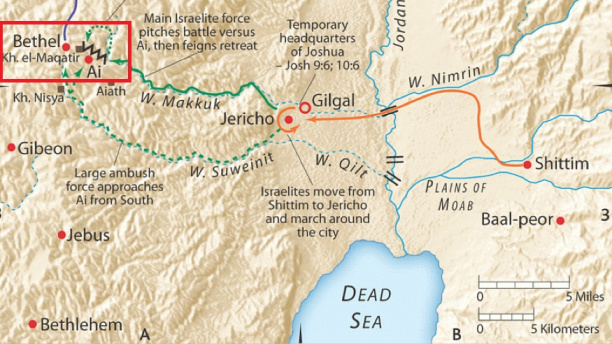
\includegraphics[width=1.05\linewidth]{BLiShiFigs/betheAi}
  %\caption{A subfigure}
  \label{fig:sub1}
\end{subfigure}%
\hspace*{5mm}
\vspace*{-8mm}
\begin{subfigure}{.5\textwidth}
  \centering
  \includegraphics[width=.93\linewidth]{BLiShiFigs/aiWar}
 % \caption{A subfigure}
  \label{fig:sub2}
\end{subfigure}
\caption{攻打艾城}
\label{fig:test}
\end{figure}
\begin{itemize}
\item The main Israelite force of 25,000 advanced to a point north of Ai, well within sight of the city with a valley between them and the city.
\item Meanwhile, an elite detachment of 5,000 gathered in the rear for executing an ambush, positioned west of Ai (between Bethel and Ai)
\item The main body advanced seemingly for another frontal assault as before
\item As the King of Ai delivered a spoiling attack 3, the Israelites feigned a retreat, as had happened in the earlier assault, and retreated
\item This maneuver lured every Canaanite soldier of Ai and Bethel out into the open deep gorge (Wadi Muheisin) in pursuit of the retreating Israelite attack
\item The rear ambush force entered the city and set it ablaze
\item The two groups made up of the ambush force, and the main body turned around again towards the Aians, effectively trapping them in a vic
\item Another detachment had been deployed to block any assistance sent from Bethel to help Ai.
\end{itemize}

於是，約書亞和一切兵丁都起來，要上艾城去。約書亞選了三萬大能的勇士，夜間打發他們前往， 4 吩咐他們說：「你們要在城後埋伏，不可離城太遠，都要各自準備。 5 我與我所帶領的眾民要向城前往。城裡的人像初次出來攻擊我們的時候，我們就在他們面前逃跑， 6 他們必出來追趕我們，直到我們引誘他們離開城，因為他們必說：『這些人像初次在我們面前逃跑。』所以我們要在他們面前逃跑， 7 你們就從埋伏的地方起來，奪取那城，因為耶和華你們的神必把城交在你們手裡。 8 你們奪了城以後，就放火燒城，要照耶和華的話行。這是我吩咐你們的。」 9 約書亞打發他們前往，他們就上埋伏的地方去，住在伯特利和艾城的中間，就是在艾城的西邊。這夜約書亞卻在民中住宿。


\subsubsection{約書亞清早在艾城北邊安營 8:10-11}
約書亞清早起來，點齊百姓，他和以色列的長老在百姓前面上艾城去。 11 眾民，就是他所帶領的兵丁，都上去，向前直往，來到城前，在艾城北邊安營。

\subsubsection{艾城的西邊布兵五千 8:11-12}
在約書亞和艾城中間有一山谷。 12 他挑了約有五千人，使他們埋伏在伯特利和艾城的中間，就是在艾城的西邊。

\subsubsection{約書亞和以色列眾人在艾城面前裝敗 8:13-17}
於是安置了百姓，就是城北的全軍和城西的伏兵。這夜約書亞進入山谷之中。 14 艾城的王看見這景況，就和全城的人清早急忙起來，按所定的時候，出到亞拉巴前，要與以色列人交戰。王卻不知道在城後有伏兵。 15 約書亞和以色列眾人在他們面前裝敗，往那通曠野的路逃跑。 16 城內的眾民都被招聚，追趕他們。艾城人追趕的時候，就被引誘離開城。 17 艾城和伯特利城沒有一人不出來追趕以色列人的，撇了敞開的城門，去追趕以色列人。

\subsubsection{以色列取艾城而焚之 8:18-29}
耶和華吩咐約書亞說：「你向艾城伸出手裡的短槍，因為我要將城交在你手裡。」約書亞就向城伸出手裡的短槍。 19 他一伸手，伏兵就從埋伏的地方急忙起來，奪了城，跑進城去，放火焚燒。 20 艾城的人回頭一看，不料，城中煙氣沖天，他們就無力向左向右逃跑。那往曠野逃跑的百姓便轉身攻擊追趕他們的人。 21 約書亞和以色列眾人見伏兵已經奪了城，城中煙氣飛騰，就轉身回去，擊殺艾城的人。 22 伏兵也出城迎擊艾城人。艾城人就困在以色列人中間，前後都是以色列人。於是以色列人擊殺他們，沒有留下一個，也沒有一個逃脫的， 23 生擒了艾城的王，將他解到約書亞那裡。

以色列人在田間和曠野殺盡所追趕一切艾城的居民。艾城人倒在刀下，直到滅盡。以色列眾人就回到艾城，用刀殺了城中的人。 25 當日殺斃的人，連男帶女共有一萬二千，就是艾城所有的人。 26 約書亞沒有收回手裡所伸出來的短槍，直到把艾城的一切居民盡行殺滅。 27 唯獨城中的牲畜和財物，以色列人都取為自己的掠物，是照耶和華所吩咐約書亞的話。 28 約書亞將艾城焚燒，使城永為高堆、荒場，直到今日。 29 又將艾城王掛在樹上，直到晚上。日落的時候，約書亞吩咐人把屍首從樹上取下來，丟在城門口，在屍首上堆成一大堆石頭，直存到今日。

\subsubsection{基利心山以巴路山宣讀祝福咒詛 8:30-35}
那時，約書亞在以巴路山上為耶和華以色列的神築一座壇， 31 是用沒有動過鐵器的整石頭築的，照著耶和華僕人摩西所吩咐以色列人的話，正如摩西律法書上所寫的。眾人在這壇上給耶和華奉獻燔祭和平安祭。 32 約書亞在那裡，當著以色列人面前，將摩西所寫的律法抄寫在石頭上。 33 以色列眾人，無論是本地人是寄居的，和長老、官長並審判官都站在約櫃兩旁，在抬耶和華約櫃的祭司利未人面前，一半對著基利心山，一半對著以巴路山，為以色列民祝福，正如耶和華僕人摩西先前所吩咐的。 34 隨後約書亞將律法上祝福、咒詛的話，照著律法書上一切所寫的，都宣讀了一遍。 35 摩西所吩咐的一切話，約書亞在以色列全會眾和婦女、孩子，並他們中間寄居的外人面前，沒有一句不宣讀的。



\subsection{解圍基遍並擊殺五王 9-10 }

\subsubsection{諸王會盟謀攻以色列人 9:1-2 }
約旦河西住山地、高原，並對著黎巴嫩山沿大海一帶的諸王，就是赫人、亞摩利人、迦南人、比利洗人、希未人、耶布斯人的諸王，聽見這事， 2 就都聚集，同心合意地要與約書亞和以色列人爭戰。

\subsubsection{基遍人用騙取手段與以色列人立約 9:3-15}
基遍的居民聽見約書亞向耶利哥和艾城所行的事， 4 就設詭計，假充使者，拿舊口袋和破裂縫補的舊皮酒袋馱在驢上， 5 將補過的舊鞋穿在腳上，把舊衣服穿在身上。他們所帶的餅都是乾的，長了霉了。 6 他們到吉甲營中見約書亞，對他和以色列人說：「我們是從遠方來的，現在求你與我們立約。」 7 以色列人對這些希未人說：「只怕你們是住在我們中間的，若是這樣，怎能和你們立約呢？」 8 他們對約書亞說：「我們是你的僕人。」約書亞問他們說：「你們是什麼人？是從哪裡來的？」 9 他們回答說：「僕人從極遠之地而來，是因聽見耶和華你神的名聲和他在埃及所行的一切事， 10 並他向約旦河東的兩個亞摩利王，就是希實本王西宏和在亞斯他錄的巴珊王噩一切所行的事。 11 我們的長老和我們那地的一切居民對我們說：「你們手裡要帶著路上用的食物去迎接以色列人，對他們說：『我們是你們的僕人，現在求你們與我們立約。』 12 我們出來要往你們這裡來的日子，從家裡帶出來的這餅還是熱的，看哪，現在都乾了，長了霉了。 13 這皮酒袋，我們盛酒的時候還是新的，看哪，現在已經破裂。我們這衣服和鞋，因為道路甚遠，也都穿舊了。」 14 以色列人受了他們些食物，並沒有求問耶和華。 15 於是約書亞與他們講和，與他們立約，容他們活著。會眾的首領也向他們起誓。

\subsubsection{咒詛基遍人為神的殿劈柴挑水 9:16-27}
以色列人與他們立約之後，過了三天才聽見他們是近鄰，住在以色列人中間的。 17 以色列人起行，第三天到了他們的城邑，就是基遍、基非拉、比錄、基列耶琳。 18 因為會眾的首領已經指著耶和華以色列的神向他們起誓，所以以色列人不擊殺他們。全會眾就向首領發怨言。 19 眾首領對全會眾說：「我們已經指著耶和華以色列的神向他們起誓，現在我們不能害他們。 20 我們要如此待他們，容他們活著，免得有憤怒因我們所起的誓臨到我們身上。」 21 首領又對會眾說：「要容他們活著。」於是他們為全會眾做了劈柴挑水的人，正如首領對他們所說的話。

約書亞召了他們來，對他們說：「為什麼欺哄我們說我們離你們甚遠呢？其實你們是住在我們中間。 23 現在你們是被咒詛的。你們中間的人必斷不了做奴僕，為我神的殿做劈柴挑水的人。」 24 他們回答約書亞說：「因為有人實在告訴你的僕人，耶和華你的神曾吩咐他的僕人摩西，把這全地賜給你們，並在你們面前滅絕這地的一切居民，所以我們為你們的緣故甚怕喪命，就行了這事。 25 現在我們在你手中，你以怎樣待我們為善為正，就怎樣做吧！」 26 於是約書亞這樣待他們，救他們脫離以色列人的手，以色列人就沒有殺他們。 27 當日約書亞使他們在耶和華所要選擇的地方，為會眾和耶和華的壇做劈柴挑水的人，直到今日。

\subsubsection{五王合攻基遍 10:1-5}
\begin{wraptable}{r}{5cm}
\centering
\begin{tabular}{|c|c|}
\hline
\hline
地點 & 名稱   \\\hline
耶路撒冷王 & 亞多尼洗德   \\\hline
希伯崙王&何咸  \\\hline
耶末王&毗蘭  \\\hline
拉吉王&　雅非亞　\\\hline
伊磯倫王&底璧　\\\hline
\end{tabular}
\caption{五個亞摩利王}
\end{wraptable}
耶路撒冷王亞多尼洗德聽見約書亞奪了艾城，盡行毀滅，怎樣待耶利哥和耶利哥的王，也照樣待艾城和艾城的王，又聽見基遍的居民與以色列人立了和約，住在他們中間， 2 就甚懼怕。因為基遍是一座大城，如都城一般，比艾城更大，並且城內的人都是勇士。 3 所以耶路撒冷王亞多尼洗德打發人去見希伯崙王何咸、耶末王毗蘭、拉吉王雅非亞和伊磯倫王底璧，說： 4 「求你們上來幫助我，我們好攻打基遍，因為他們與約書亞和以色列人立了和約。」 5 於是五個亞摩利王，就是耶路撒冷王、希伯崙王、耶末王、拉吉王、伊磯倫王，大家聚集，率領他們的眾軍上去，對著基遍安營，攻打基遍。

\subsubsection{基遍求助，約書亞出手幫助 10:6-9}
基遍人就打發人往吉甲的營中去見約書亞，說：「你不要袖手不顧你的僕人，求你速速上來拯救我們，幫助我們，因為住山地亞摩利人的諸王都聚集攻擊我們。」於是約書亞和他一切兵丁，並大能的勇士，都從吉甲上去。 8 耶和華對約書亞說：「不要怕他們，因為我已將他們交在你手裡，他們無一人能在你面前站立得住。」 9 約書亞就終夜從吉甲上去，猛然臨到他們那裡。


\subsubsection{耶和華幫助以色列擊殺五王 10:10-14}
\begin{wrapfigure}{r}{0.6\textwidth} 
\vspace{-20pt}
\center
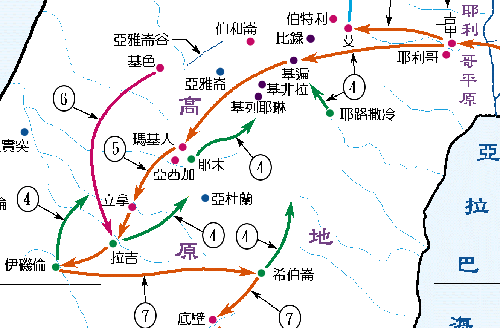
\includegraphics[width=0.6\textwidth]{BLiShiFigs/fiveKings3}
\caption{五個亞摩利王}
\end{wrapfigure} 
耶和華使他們在以色列人面前潰亂。約書亞在基遍大大地殺敗他們，追趕他們，在伯和崙的上坡路擊殺他們，直到亞西加和瑪基大。 11 他們在以色列人面前逃跑，正在伯和崙下坡的時候，耶和華從天上降大冰雹(石頭)在他們身上，直降到亞西加，打死他們。被冰雹打死的，比以色列人用刀殺死的還多。當耶和華將亞摩利人交付以色列人的日子，約書亞就禱告耶和華，在以色列人眼前說：「日頭啊，你要停在基遍！月亮啊，你要止在亞雅崙谷！」 13 於是日頭停留，月亮止住，直等國民向敵人報仇。這事豈不是寫在《雅煞珥書》上嗎？「日頭在天當中停住，不急速下落，約有一日之久。」 14 在這日以前，這日以後，耶和華聽人的禱告沒有像這日的，是因耶和華為以色列爭戰。


\subsubsection{捉拿五王 10:15-21}
約書亞和以色列眾人回到吉甲的營中。
那五王逃跑，藏在瑪基大洞裡。有人告訴約書亞說：「那五王已經找到了，都藏在瑪基大洞裡。」約書亞說：「你們把幾塊大石頭滾到洞口，派人看守。你們卻不可耽延，要追趕你們的仇敵，擊殺他們儘後邊的人，不容他們進自己的城邑，因為耶和華你們的神已經把他們交在你們手裡。」約書亞和以色列人大大殺敗他們，直到將他們滅盡，其中剩下的人都進了堅固的城。 眾百姓就安然回瑪基大營中，到約書亞那裡。沒有一人敢向以色列人饒舌。

\subsubsection{擊殺五王 10:22-27}
\begin{table}[H]
\begin{tabular}{ p{10.cm}|p{7.cm}} \toprule
\toprule
約書亞 &眾人 \\\hline
約書亞說：「打開洞口，將那五王從洞裡帶出來，領到我面前。」 &眾人就這樣行，將那五王，就是耶路撒冷王、希伯崙王、耶末王、拉吉王、伊磯倫王，從洞裡帶出來，領到約書亞面前。\tabularnewline\hline
帶出那五王到約書亞面前的時候，約書亞就召了以色列眾人來，對那些和他同去的軍長說：「你們近前來，把腳踏在這些王的頸項上。」&他們就近前來，把腳踏在這些王的頸項上。\tabularnewline\hline
約書亞對他們說：「你們不要懼怕，也不要驚惶。應當剛強壯膽，因為耶和華必這樣待你們所要攻打的一切仇敵。」隨後約書亞將這五王殺死，掛在五棵樹上。 & 他們就在樹上直掛到晚上。\tabularnewline\hline
日頭要落的時候，約書亞一吩咐，&人就把屍首從樹上取下來，丟在他們藏過的洞裡，把幾塊大石頭放在洞口，直存到今日。 \tabularnewline
\hline\bottomrule
\end{tabular}
\caption{擊殺五王}
\end{table} 


   
\subsubsection{攻打其他的城邑 10:28-39}
\begin{wraptable}{r}{10cm}
\vspace*{-10mm}
\centering
\begin{tabular}{|c|c|}
\hline
\hline
地點 & 事件  \\\hline
瑪基大 & 殺死五個亞摩利王   \\\hline
立拿&殺死立拿王,和城中的一切人口  \\\hline
拉吉&殺死城中的一切人口,和基色王荷蘭  \\\hline
伊磯倫&　殺死城中的一切人口　\\\hline
希伯崙&殺死城中的人與王，並那些城邑中的人口　\\\hline
底璧&殺死底璧的王和屬底璧的城邑中的人口　\\\hline
\end{tabular}
\caption{攻打周圍的王}
\end{wraptable}
當日，約書亞奪了瑪基大，用刀擊殺城中的人和王，將其中一切人口盡行殺滅，沒有留下一個。他待瑪基大王像從前待耶利哥王一樣。

29 約書亞和以色列眾人從瑪基大往立拿去，攻打立拿。 30 耶和華將立拿和立拿的王也交在以色列人手裡。約書亞攻打這城，用刀擊殺了城中的一切人口，沒有留下一個。他待立拿王像從前待耶利哥王一樣。

31 約書亞和以色列眾人從立拿往拉吉去，對著拉吉安營，攻打這城。 32 耶和華將拉吉交在以色列人的手裡。第二天約書亞就奪了拉吉，用刀擊殺了城中的一切人口，是照他向立拿一切所行的。

33 那時基色王荷蘭上來幫助拉吉，約書亞就把他和他的民都擊殺了，沒有留下一個。

34 約書亞和以色列眾人從拉吉往伊磯倫去，對著伊磯倫安營，攻打這城。 35 當日就奪了城，用刀擊殺了城中的人。那日，約書亞將城中的一切人口盡行殺滅，是照他向拉吉一切所行的。

36 約書亞和以色列眾人從伊磯倫上希伯崙去，攻打這城， 37 就奪了希伯崙和屬希伯崙的諸城邑，用刀將城中的人與王，並那些城邑中的人口，都擊殺了，沒有留下一個，是照他向伊磯倫所行的，把城中的一切人口盡行殺滅。
 約書亞和以色列眾人回到底璧，攻打這城， 39 就奪了底璧和屬底璧的城邑，又擒獲底璧的王，用刀將這些城中的人口盡行殺滅，沒有留下一個。他待底璧和底璧王，像從前待希伯崙和立拿與立拿王一樣。

\subsubsection{擊殺山地、南地、高原、山坡諸王 10:40-43}
這樣，約書亞擊殺全地的人，就是山地、南地、高原、山坡的人和那些地的諸王，沒有留下一個。將凡有氣息的盡行殺滅，正如耶和華以色列的神所吩咐的。 41 約書亞從加低斯巴尼亞攻擊到加沙，又攻擊歌珊全地，直到基遍。 42 約書亞一時殺敗了這些王，並奪了他們的地，因為耶和華以色列的神為以色列爭戰。 43 於是約書亞和以色列眾人回到吉甲的營中。
\sffamily\begin{tikzpicture}
  \matrix (m) [matrix of nodes, 
    column sep=5mm,
    row sep=1cm,
    nodes={draw, % General options for all nodes
      line width=1pt,
      anchor=center, 
      text centered,
      rounded corners,
      minimum width=1.5cm, minimum height=8mm
    }, 
    % Define styles for some special nodes
    right iso/.style={isosceles triangle,scale=0.5,sharp corners, anchor=center, xshift=-4mm},
    left iso/.style={right iso, rotate=180, xshift=-8mm},
    txt/.style={text width=1.5cm,anchor=center},
    ellip/.style={ellipse,scale=0.5},
    empty/.style={draw=none}
    ]   
  {
  % m-1-1
    加低斯巴尼亞
  & % m-1-2
    迦薩
  & % m-1-3
    歌珊全地
  & % m-1-4
    基遍   
      \\     
  };  % End of matrix
{ [start chain,every on chain/.style={join}, every join/.style={line width=1pt}]
  	 \chainin (m-1-1);
    \chainin (m-1-2);
    \chainin (m-1-3); 
    \chainin (m-1-4);                   
    };
\end{tikzpicture}  

\subsection{其他的戰役 11-12 }

\subsubsection{北方耶賓會合諸王與以色列人爭戰 11:1-5}
\begin{table}[H]
\centering
\begin{tabular}{|c|c|}
\hline
\hline
地點 & 名稱  \\\hline
夏瑣王 & 耶賓 \\\hline
北方山地、基尼烈南邊的亞拉巴高原&   \\\hline
西邊多珥山岡&諸王  \\\hline
東方的迦南人&　 　\\\hline
西方的迦南人& 　\\\hline
山地的亞摩利人、赫人、比利洗人、耶布斯人& 　\\\hline
黑門山根米斯巴地的希未人& 　\\\hline
\end{tabular}
\caption{北方諸王與以色列人爭戰}
\end{table}
夏瑣王耶賓聽見這事，就打發人去見瑪頓王約巴、伸崙王、押煞王， 2 與北方山地、基尼烈南邊的亞拉巴高原並西邊多珥山岡的諸王。 3 又去見東方和西方的迦南人，與山地的亞摩利人、赫人、比利洗人、耶布斯人，並黑門山根米斯巴地的希未人。 4 這些王和他們的眾軍都出來，人數多如海邊的沙，並有許多馬匹車輛。 5 這諸王會合，來到米倫水邊，一同安營，要與以色列人爭戰。

\subsubsection{被神勉励，約書亞率兵爭戰 11:6-9}
耶和華對約書亞說：「你不要因他們懼怕，明日這時，我必將他們交付以色列人全然殺了。你要砍斷他們馬的蹄筋，用火焚燒他們的車輛。」於是約書亞率領一切兵丁，在米倫水邊突然向前攻打他們。耶和華將他們交在以色列人手裡，以色列人就擊殺他們，追趕他們到西頓大城，到米斯利弗瑪音，直到東邊米斯巴的平原，將他們擊殺，沒有留下一個。約書亞就照耶和華所吩咐他的去行，砍斷他們馬的蹄筋，用火焚燒他們的車輛。
  \sffamily\begin{tikzpicture}
  \matrix (m) [matrix of nodes, 
    column sep=5mm,
    row sep=1cm,
    nodes={draw, % General options for all nodes
      line width=1pt,
      anchor=center, 
      text centered,
      rounded corners,
      minimum width=1.5cm, minimum height=8mm
    }, 
    % Define styles for some special nodes
    right iso/.style={isosceles triangle,scale=0.5,sharp corners, anchor=center, xshift=-4mm},
    left iso/.style={right iso, rotate=180, xshift=-8mm},
    txt/.style={text width=1.5cm,anchor=center},
    ellip/.style={ellipse,scale=0.5},
    empty/.style={draw=none}
    ]   
  {
  % m-1-1
    米倫水邊
  & % m-1-2
  西頓大城
  & % m-1-3
   米斯利弗瑪音
  & % m-1-4
   東邊米斯巴的平原   
   &夏瑣
      \\     
  };  % End of matrix
  { [start chain,every on chain/.style={join}, every join/.style={line width=1pt}]
  	 \chainin (m-1-1);
    \chainin (m-1-2);
    \chainin (m-1-3); 
    \chainin (m-1-4);    \chainin (m-1-5);                   
    };
\end{tikzpicture}  

\subsubsection{戰败联军，焚烧夏瑣 11:10-15}
當時，約書亞轉回奪了夏瑣，用刀擊殺夏瑣王，素來夏瑣在這諸國中是為首的。 11 以色列人用刀擊殺城中的人口，將他們盡行殺滅，凡有氣息的沒有留下一個。約書亞又用火焚燒夏瑣。 12 約書亞奪了這些王的一切城邑，擒獲其中的諸王，用刀擊殺他們，將他們盡行殺滅，正如耶和華僕人摩西所吩咐的。 13 至於造在山岡上的城，除了夏瑣以外，以色列人都沒有焚燒。約書亞只將夏瑣焚燒了。 14 那些城邑所有的財物和牲畜，以色列人都取為自己的掠物。唯有一切人口都用刀擊殺，直到殺盡，凡有氣息的沒有留下一個。 15 耶和華怎樣吩咐他僕人摩西，摩西就照樣吩咐約書亞，約書亞也照樣行。凡耶和華所吩咐摩西的，約書亞沒有一件懈怠不行的。

\subsubsection{約書亞攻取之地 11:16-20}
約書亞奪了那全地，就是山地、一帶南地、歌珊全地、高原、亞拉巴、以色列的山地和山下的高原，從上西珥的哈拉山，直到黑門山下黎巴嫩平原的巴力迦得，並且擒獲那些地的諸王，將他們殺死。約書亞和這諸王爭戰了許多年日。除了基遍的希未人之外，沒有一城與以色列人講和的，都是以色列人爭戰奪來的。因為耶和華的意思是要使他們心裡剛硬，來與以色列人爭戰，好叫他們盡被殺滅，不蒙憐憫，正如耶和華所吩咐摩西的。

\subsubsection{在以色列人的地剪除了亞衲族人 11:21-23}
當時約書亞來到，將住山地、希伯崙、底璧、亞拿伯、猶大山地、以色列山地所有的亞衲族人剪除了。約書亞將他們和他們的城邑盡都毀滅。在以色列人的地沒有留下一個亞衲族人，只在加沙、迦特和亞實突有留下的。這樣，約書亞照著耶和華所吩咐摩西的一切話奪了那全地，就按著以色列支派的宗族將地分給他們為業。於是國中太平，沒有爭戰了。

\subsection{擊殺的諸王 12 }
\subsubsection{摩西擊殺的王，2個 12:1-6}
\newcolumntype{L}{>{\centering\arraybackslash}m{3cm}}
\begin{table}[H]
\centering
\begin{tabular}{|c|c|c|}
\hline
\hline
名稱 & 地點 &範圍 \\\hline
西宏&\multicolumn{1}{m{2cm}|}{希實本、亞摩利人的王}& \multicolumn{1}{m{12cm}|}{他所管之地是從亞嫩谷邊的亞羅珥和谷中的城，並基列一半，直到亞捫人的境界，與約但河東邊的亞拉巴，直到基尼烈海，又到亞拉巴的海，就是鹽海，通伯耶西末的路，以及南方，直到毗斯迦的山根。} \\\hline
噩  &\multicolumn{1}{m{2cm}|}{利乏音人所剩下的，住在亞斯他錄和以得來的巴珊王}&\multicolumn{1}{m{12cm}|}{黑門山、撒迦、巴珊全地，直到基述人和瑪迦人的境界，並基列一半，直到希實本王西宏的境界。} \\\hline
\end{tabular}
\caption{摩西擊殺的王,2個}
\end{table}
以色列人在約旦河外向日出之地擊殺二王，得他們的地，就是從亞嫩谷直到黑門山，並東邊的全亞拉巴之地。 2 這二王，有住希實本亞摩利人的王西宏。他所管之地是：從亞嫩谷邊的亞羅珥和谷中的城，並基列一半，直到亞捫人的境界雅博河； 3 與約旦河東邊的亞拉巴，直到基尼烈海，又到亞拉巴的海，就是鹽海，通伯耶西末的路；以及南方，直到毗斯迦的山根。 4 又有巴珊王噩，他是利乏音人所剩下的，住在亞斯他錄和以得來。 5 他所管之地是：黑門山，撒迦，巴珊全地，直到基述人和瑪迦人的境界，並基列一半，直到希實本王西宏的境界。 6 這二王是耶和華僕人摩西和以色列人所擊殺的。耶和華僕人摩西將他們的地賜給魯本人、迦得人和瑪拿西半支派的人為業。

\subsubsection{約書亞擊殺的王,31個 12:7-24}
 \begin{table}[H]
\centering
\begin{tabular}{|c|c|c|c|}
\hline
\hline
耶利哥王&靠近伯特利的艾城王 & 耶路撒冷王& 希伯崙王 \\\hline
耶末王&拉吉王& 伊磯倫王&基色王 \\\hline
底璧王&基德王& 何珥瑪王 &亞拉得王  \\\hline
立拿王&亞杜蘭王 &瑪基大王&伯特利王  \\\hline
他普亞王&希弗王& 亞弗王&拉沙崙王 \\\hline
瑪頓王&夏瑣王 &伸崙米崙王&押煞王 \\\hline
他納王&米吉多王 &基低斯王&靠近迦密的約念王 \\\hline
多珥山岡的多珥王&吉甲的戈印王 &得撒王 & \\\hline
\end{tabular}
\caption{約書亞擊殺的王,31個}
\end{table}
約書亞和以色列人在約旦河西擊殺了諸王。他們的地是從黎巴嫩平原的巴力迦得，直到上西珥的哈拉山。約書亞就將那地按著以色列支派的宗族分給他們為業， 8 就是赫人、亞摩利人、迦南人、比利洗人、希未人、耶布斯人的山地、高原亞拉巴、山坡、曠野和南地。 9 他們的王，一個是耶利哥王，一個是靠近伯特利的艾城王， 10 一個是耶路撒冷王，一個是希伯崙王， 11 一個是耶末王，一個是拉吉王， 12 一個是伊磯倫王，一個是基色王， 13 一個是底璧王，一個是基德王， 14 一個是何珥瑪王，一個是亞拉得王， 15 一個是立拿王，一個是亞杜蘭王， 16 一個是瑪基大王，一個是伯特利王， 17 一個是他普亞王，一個是希弗王， 18 一個是亞弗王，一個是拉沙崙王， 19 一個是瑪頓王，一個是夏瑣王， 20 一個是伸侖米崙王，一個是押煞王， 21 一個是他納王，一個是米吉多王， 22 一個是基低斯王，一個是靠近迦密的約念王， 23 一個是多珥山岡的多珥王，一個是吉甲的戈印王， 24 一個是得撒王，共計三十一個王。

%\newpage
\section{以色列人分地 13-21 }
\subsection{未得之地 13:1-7}
\subsubsection{耶和華命為九個半支派分地 13:1-7}
約書亞年紀老邁，耶和華對他說：「你年紀老邁了，還有許多未得之地， 2 就是非利士人的全境和基述人的全地： 3 從埃及前的西曷河往北，直到以革倫的境界，就算屬迦南人之地，有非利士人五個首領所管的加沙人、亞實突人、亞實基倫人、迦特人、以革倫人之地，並有南方亞衛人之地。 4 又有迦南人的全地，並屬西頓人的米亞拉到亞弗，直到亞摩利人的境界。 5 還有迦巴勒人之地，並向日出的全黎巴嫩，就是從黑門山根的巴力迦得，直到哈馬口。 6 山地的一切居民，從黎巴嫩直到米斯利弗瑪音，就是所有的西頓人，我必在以色列人面前趕出他們去。你只管照我所吩咐的，將這地拈鬮分給以色列人為業。 7 現在你要把這地分給九個支派和瑪拿西半個支派為業。」

\subsection{河東之地的分配 13:8-33 }
\subsubsection{二個支派半支派的范围 13:8-13 }
瑪拿西那半支派和魯本、迦得二支派已經受了產業，就是耶和華的僕人摩西在約旦河東所賜給他們的， 9 是從亞嫩谷邊的亞羅珥和谷中的城，並米底巴的全平原，直到底本； 10 和在希實本做王亞摩利王西宏的諸城，直到亞捫人的境界； 11 又有基列地，基述人、瑪迦人的地界，並黑門全山，巴珊全地，直到撒迦； 12 又有巴珊王噩的全國，他在亞斯他錄和以得來做王（利乏音人所存留的只剩下他）。這些地的人都是摩西所擊殺、所趕逐的。 13 以色列人卻沒有趕逐基述人、瑪迦人，這些人仍住在以色列中，直到今日。

\subsubsection{利未支派沒有產業 13:14}
只是利未支派，摩西（他）沒有把產業分給他們，他們的產業乃是獻於耶和華以色列神的火祭，正如耶和華所應許他們的。

\subsubsection{流便產業 13:15-23}
\begin{table}[!hbp]
\centering
\begin{tabular}{|p{15cm}|}
\hline
\hline
 亞嫩谷邊的亞羅珥和谷中的城，靠近米底巴的全平原  \\\hline
 希實本並屬希實本平原的各城，底本、巴末巴力、伯巴力勉、雅雜、基底莫、米法押、列亭、西比瑪、谷中山的細列哈沙轄、伯毗珥、毗斯迦山坡、伯耶西末\\\hline
 原的各城，並亞摩利王西宏的全國\\\hline
 \end{tabular}
\caption{河東流便支派}
\end{table}
摩西按著流便支派的宗族分給他們產業。 16 他們的境界是亞嫩谷邊的亞羅珥和谷中的城，靠近米底巴的全平原； 17 希實本並屬希實本平原的各城，底本，巴末巴力，伯巴力勉， 18 雅雜，基底莫，米法押， 19 基列亭，西比瑪，谷中山的細列哈沙轄， 20 伯毗珥，毗斯迦山坡，伯耶西末； 21 平原的各城，並亞摩利王西宏的全國。這西宏曾在希實本做王，摩西把他和米甸的族長以未、利金、蘇珥、戶珥、利巴擊殺了。這都是住那地屬西宏為首領的。 22 那時以色列人在所殺的人中，也用刀殺了比珥的兒子術士巴蘭。 23 魯本人的境界就是約旦河與靠近約旦河的地。以上是魯本人按著宗族所得為業的諸城，並屬城的村莊。


\subsubsection{迦得產業 13:24-28}
\begin{table}[!hbp]
\centering
\begin{tabular}{|p{15cm}|}
\hline
\hline
 雅謝和基列的各城，並亞捫人的一半地，直到拉巴前的亞羅珥； \\\hline
 從希實本到拉抹米斯巴和比多寧，又從瑪哈念到底璧的境界\\\hline
 並谷中的伯亞蘭、伯寧拉、疏割、撒分，就是希實本王西宏國中的餘地\\\hline
 以及約但河與靠近約但河的地，直到基尼烈海的極邊，都在約但河東\\\hline
 \end{tabular}
\caption{河東迦得支派}
\end{table}
摩西按著迦得支派的宗族分給他們產業。 25 他們的境界是雅謝和基列的各城，並亞捫人的一半地，直到拉巴前的亞羅珥； 26 從希實本到拉抹米斯巴和比多寧，又從瑪哈念到底璧的境界， 27 並谷中的伯亞蘭、伯寧拉、疏割、撒分，就是希實本王西宏國中的餘地；以及約旦河與靠近約旦河的地，直到基尼烈海的極邊，都在約旦河東。 28 以上是迦得人按著宗族所得為業的諸城，並屬城的村莊。

\subsubsection{瑪拿西半支派的產業 13:29-31}
\begin{table}[H]
\centering
\begin{tabular}{|c|c|}
\hline
\hline
 從瑪哈念起 &包括巴珊全地，就是巴珊王噩的全國，並在巴珊、睚珥的一切城邑，共六十個  \\\hline
 基列的一半 &並亞斯他錄、以得來，就是屬巴珊王噩國的二城，\\\hline
 \end{tabular}
\caption{河東瑪拿西半支派}
\end{table}

\subsubsection{以色列的神是利未支派的產業 13:32-33}
以上是摩西在約旦河東對著耶利哥的摩押平原所分給他們的產業。只是利未支派，摩西沒有把產業分給他們，耶和華以色列的神是他們的產業，正如耶和華所應許他們的。

\subsection{河西之地的分配 14-19 }
\subsubsection{综述九個半支派的地 14:1-2}
以色列人在迦南地所得的產業，就是祭司以利亞撒和嫩的兒子約書亞並以色列各支派的族長所分給他們的，都記在下面，是照耶和華藉摩西所吩咐的，把產業拈鬮分給九個半支派。

\subsubsection{利未人沒有產業 14:3-5}
原來摩西在約旦河東已經把產業分給那兩個半支派，只是在他們中間沒有把產業分給利未人。因為約瑟的子孫是兩個支派，就是瑪拿西和以法蓮，所以沒有把地分給利未人，但給他們城邑居住，並城邑的郊野，可以牧養他們的牲畜，安置他們的財物。耶和華怎樣吩咐摩西，以色列人就照樣行，把地分了。

\subsubsection{迦勒向約書亞求希伯崙為業 14:6-15}
\begin{table}[H]
\centering
\begin{tabular}{p{15.7cm}|p{1.18cm}}\hline\hline
迦勒&約書亞\\\hline
那時，猶大人來到吉甲見約書亞，有基尼洗族耶孚尼的兒子迦勒對約書亞說：「耶和華在加低斯巴尼亞指著我與你對神人摩西所說的話，你都知道了。耶和華的僕人摩西從加低斯巴尼亞打發我窺探這地，那時我正四十歲，我按著心意回報他。然而同我上去的眾弟兄使百姓的心消化，但我專心跟從耶和華我的神。當日摩西起誓說：『你腳所踏之地定要歸你和你的子孫永遠為業，因為你專心跟從耶和華我的神。』自從耶和華對摩西說這話的時候，耶和華照他所應許的，使我存活這四十五年，其間以色列人在曠野行走。看哪，現今我八十五歲了，我還是強壯，像摩西打發我去的那天一樣。無論是爭戰是出入，我的力量那時如何，現在還是如何。求你將耶和華那日應許我的這山地給我。那裡有亞衲族人，並寬大堅固的城，你也曾聽見了。或者耶和華照他所應許的與我同在，我就把他們趕出去。」
&於是約書亞為耶孚尼的兒子迦勒祝福將希伯崙給他為業。\\\hline
所以希伯崙做了基尼洗族耶孚尼的兒子迦勒的產業，直到今日，因為他專心跟從耶和華以色列的神。希伯崙從前名叫基列亞巴，亞巴是亞衲族中最尊大的人。於是國中太平，沒有爭戰了。&\\\hline
 \end{tabular}
\caption{迦勒向約書亞求希伯崙為業}
\end{table}




\subsubsection{猶大所得之地 15:1-12}
\begin{table}[H]
\centering
\begin{tabular}{p{4.7cm}|p{0.79cm}|p{8.7cm}|p{1.5cm}}\hline\hline
南界&東界&北界&西界\\\hline
猶大支派按著宗族拈鬮所得之地是在儘南邊，到以東的交界，向南直到尋的曠野。他們的南界是從鹽海的儘邊，就是從朝南的海汊起，通到亞克拉濱坡的南邊，接連到尋，上到加低斯巴尼亞的南邊，又過希斯崙，上到亞達珥，繞到甲加，接連到押們，通到埃及小河，直通到海為止。這就是他們的南界。 
&東界是從鹽海南邊到約旦河口。
&北界是從約旦河口的海汊起，上到伯曷拉，過伯亞拉巴的北邊，上到魯本之子波罕的磐石；從亞割谷往北，上到底璧，直向河南亞都冥坡對面的吉甲；又接連到隱示麥泉，直通到隱羅結，上到欣嫩子谷，貼近耶布斯的南界（耶布斯就是耶路撒冷）；又上到欣嫩谷西邊的山頂，就是在利乏音谷極北的邊界；又從山頂延到尼弗多亞的水源，通到以弗崙山的城邑，又延到巴拉（巴拉就是基列耶琳），又從巴拉往西繞到西珥山，接連到耶琳山的北邊（耶琳就是基撒崙）；又下到伯示麥過亭納，通到以革倫北邊，延到施基崙，接連到巴拉山，又通到雅比聶，直通到海為止。
&西界就是大海和靠近大海之地。這是猶大人按著宗族所得之地四圍的交界。\\\hline
 \end{tabular}
\caption{猶大所得之地}
\end{table}


\subsubsection{俄陀聶攻取基列西弗得迦勒女兒為妻 14:13-19}
\begin{table}[H]
\centering
\begin{tabular}{p{4.cm}|p{5.2cm}|p{1.7cm}|p{5.cm}}\hline\hline
約書亞&迦勒&俄陀聶&押撒\\\hline
約書亞照耶和華所吩咐的，將猶大人中的一段地，就是基列亞巴，分給耶孚尼的兒子迦勒；亞巴是亞衲族的始祖，基列亞巴就是希伯崙。
&迦勒就從那裡趕出亞衲族的三個族長，就是示篩、亞希幔、撻買。又從那裡上去，攻擊底璧的居民，這底璧從前名叫基列西弗。迦勒說：「誰能攻打基列西弗將城奪取，我就把我女兒押撒給他為妻。」
&迦勒兄弟基納斯的兒子俄陀聶奪取了那城，
&\\\hline
&迦勒就把女兒押撒給他為妻。&&押撒過門的時候，勸丈夫向她父親求一塊田。押撒一下驢，\\\hline
&迦勒問她說：「你要什麼？」&&她說：「求你賜福給我，你既將我安置在南地，求你也給我水泉。」\\\hline
&她父親就把上泉下泉賜給她。&&\\\hline
 \end{tabular}
\caption{俄陀聶攻取基列西弗得迦勒女兒為妻}
\end{table}

\subsubsection{猶大按著宗族所得的產業 14:20-63}
以下是猶大支派按著宗族所得的產業。

猶大支派儘南邊的城邑，與以東交界相近的，就是甲薛、以得、雅姑珥、 基拿、底摩拿、亞大達、基低斯、夏瑣、以提楠、西弗、提鏈、比亞綠、夏瑣哈大他、加略希斯崙（加略希斯崙就是夏瑣）、亞曼、示瑪、摩拉大、哈薩迦大、黑實門、伯帕列、哈薩書亞、別是巴、比斯約他、巴拉、以因、以森、伊勒多臘、基失、何珥瑪、洗革拉、麥瑪拿、三撒拿、利巴勿、實忻、亞因、臨門，共二十九座城，還有屬城的村莊。

在高原有以實陶、瑣拉、亞實拿、撒挪亞、隱干寧、他普亞、以楠、耶末、亞杜蘭、梭哥、亞西加、沙拉音、亞底他音、基底拉、基底羅他音，共十四座城，還有屬城的村莊。

又有洗楠、哈大沙、麥大迦得、底連、米斯巴、約帖、拉吉、波斯加、伊磯倫、迦本、拉幔、基提利、基低羅、伯大袞、拿瑪、瑪基大，共十六座城，還有屬城的村莊。

又有立拿、以帖、亞珊、 益弗他、亞實拿、尼悉、基伊拉、亞革悉、瑪利沙，共九座城，還有屬城的村莊。

又有以革倫和屬以革倫的鎮市村莊。從以革倫直到海，一切靠近亞實突之地，並屬其地的村莊。亞實突和屬亞實突的鎮市村莊，加沙和屬加沙的鎮市村莊，直到埃及小河，並大海和靠近大海之地。

在山地有沙密、雅提珥、梭哥、大拿、基列薩拿（基列薩拿就是底璧）、亞拿伯、以實提莫、亞念、歌珊、何倫、基羅，共十一座城，還有屬城的村莊。

又有亞拉、度瑪、以珊、雅農、伯他普亞、亞非加、宏他、基列亞巴（基列亞巴就是希伯崙）、洗珥，共九座城，還有屬城的村莊。

又有瑪雲、迦密、西弗、淤他、耶斯列、約甸、撒挪亞、該隱、基比亞、亭納，共十座城，還有屬城的村莊。

又有哈忽、伯夙、基突、瑪臘、伯亞諾、伊勒提君，共六座城，還有屬城的村莊。

又有基列巴力（基列巴力就是基列耶琳）、拉巴，共兩座城，還有屬城的村莊。

在曠野有伯亞拉巴、密丁、西迦迦、匿珊、鹽城、隱基底，共六座城，還有屬城的村莊。

至於住耶路撒冷的\textcolor{red}{耶布斯人}，猶大人不能把他們趕出去，耶布斯人卻在耶路撒冷與猶大人同住，直到今日。

\subsubsection{以法連瑪拿西支派的地 16:1-10}

\begin{table}[H]
\centering
\begin{tabular}{p{6.cm}|p{6.cm}|p{2.cm}|p{2.cm}}\hline\hline
約瑟的子孫&以法蓮&瑪拿西&迦南人\\\hline
約瑟的子孫拈鬮所得之地是從靠近耶利哥的約旦河起，以耶利哥東邊的水為界，從耶利哥上去，通過山地的曠野，到伯特利；又從伯特利到路斯，接連到亞基人的境界，至亞他綠，又往西下到押利提人的境界，到下伯和崙的境界，直到基色，通到海為止。約瑟的兒子瑪拿西、以法蓮就得了他們的地業。&以法蓮子孫的境界，按著宗族所得的，記在下面。他們地業的東界是亞他綠亞達到上伯和崙；往西通到北邊的密米他，又向東繞到他納示羅，又接連到雅挪哈的東邊，從雅挪哈下到亞他綠，又到拿拉，達到耶利哥，通到約旦河為止；從他普亞往西，到加拿河，直通到海為止。這就是以法蓮支派按著宗族所得的地業。&另外在瑪拿西人地業中得了些城邑和屬城的村莊，這都是分給以法蓮子孫的。&他們沒有趕出住基色的迦南人，迦南人卻住在以法蓮人中間，成為做苦工的僕人，直到今日。\\\hline
 \end{tabular}
\caption{以法連支派的地}
\end{table}


\subsubsection{瑪拿西半支派的地 17:1-2}
瑪拿西是約瑟的長子，他的支派拈鬮所得之地記在下面。至於瑪拿西的長子基列之父(主)瑪吉，因為是勇士，就得了基列和巴珊。瑪拿西其餘的子孫，按著宗族拈鬮分地，就是亞比以謝子孫、希勒子孫、亞斯列子孫、示劍子孫、希弗子孫、示米大子孫。這些按著宗族，都是約瑟兒子瑪拿西子孫的男丁。

\subsubsection{瑪拿西半支派西羅非哈女兒的地 17:3-6}
\begin{table}[H]
\centering
\begin{tabular}{p{9.3cm}|p{8.cm}}\hline\hline
西羅非哈的女兒們&約書亞\\\hline
瑪拿西的玄孫、瑪吉的曾孫、基列的孫子、希弗的兒子西羅非哈沒有兒子只有女兒，他的女兒名叫瑪拉、挪阿、曷拉、密迦、得撒。她們來到祭司以利亞撒和嫩的兒子約書亞並眾首領面前說：「耶和華曾吩咐摩西在我們弟兄中分給我們產業。」 &於是約書亞照耶和華所吩咐的，在她們伯叔中，把產業分給她們。除了約旦河東的基列和巴珊地之外，還有十份地歸瑪拿西，因為瑪拿西的孫女們在瑪拿西的孫子中得了產業。基列地是屬瑪拿西其餘的子孫。\\\hline
 \end{tabular}
\caption{西羅非哈女兒的地 }
\end{table}


\subsubsection{瑪拿西半支派的境界 17:7-13}
\begin{table}[H]
\centering
\begin{tabular}{p{13.8cm}|p{3.34cm}}\hline\hline
瑪拿西&迦南人\\\hline
瑪拿西的境界，從亞設起，到示劍前的密米他，往北到隱他普亞居民之地。他普亞地歸瑪拿西，只是瑪拿西境界上的他普亞城歸以法蓮子孫。其界下到加拿河的南邊，在瑪拿西城邑中的這些城邑都歸以法蓮。瑪拿西的地界是在河北直通到海為止。南歸以法蓮，北歸瑪拿西，以海為界。北邊到亞設，東邊到以薩迦。瑪拿西在以薩迦和亞設境內，有伯善和屬伯善的鎮市，以伯蓮和屬以伯蓮的鎮市，多珥的居民和屬多珥的鎮市。又有三處山岡，就是隱多珥和屬隱多珥的鎮市，他納的居民和屬他納的鎮市，米吉多的居民和屬米吉多的鎮市。 &只是瑪拿西子孫不能趕出這些城的居民，迦南人偏要住在那地。及至以色列人強盛了，就使迦南人做苦工，沒有把他們全然趕出。
\\\hline
 \end{tabular}
\caption{西羅非哈女兒的地 }
\end{table}

\subsubsection{約瑟子孫和約書亞的對话 17:14-18}
\begin{table}[H]
\centering
\begin{tabular}{p{6.5cm}|p{10.5cm}}
\hline
\hline
約瑟的子孫對約書亞說：「耶和華到如今既然賜福於我們，我們也族大人多，你為什麼僅將一鬮一段之地分給我們為業呢？」 &約書亞說：「你們如果族大人多，嫌以法蓮山地窄小，就可以上比利洗人、利乏音人之地，在樹林中砍伐樹木。」 \\\hline
約瑟的子孫說：「那山地容不下我們，並且住平原的迦南人，就是住伯善和屬伯善的鎮市，並住耶斯列平原的人，都有鐵車。」&約書亞對約瑟家就是以法蓮和瑪拿西人說：「你是族大人多並且強盛，不可僅有一鬮之地。山地也要歸你，雖是樹林你也可以砍伐。靠近之地必歸你。迦南人雖有鐵車雖是強盛，你也能把他們趕出去。」\\\hline
 \end{tabular}
\caption{約瑟子孫和約書亞的對话}
\end{table}
 

\subsubsection{餘地繪圖以備鬮分 18:1-10}
\begin{table}[H]
\centering
\begin{tabular}{p{6.5cm}|p{10.5cm}}\hline\hline
以色列的全會眾&約書亞\\\hline
以色列的全會眾都聚集在示羅，把會幕設立在那裡，那地已經被他們制伏了。以色列人中其餘的七個支派還沒有分給他們地業。&約書亞對以色列人說：「耶和華你們列祖的神所賜給你們的地，你們耽延不去得，要到幾時呢？你們每支派當選舉三個人，我要打發他們去，他們就要起身走遍那地，按著各支派應得的地業寫明(畫圖)，就回到我這裡來。他們要將地分做七份。猶大仍在南方，住在他的境內。約瑟家仍在北方，住在他的境內。你們要將地分做七份，寫明了拿到我這裡來。我要在耶和華我們神面前，為你們拈鬮。利未人在你們中間沒有份，因為供耶和華祭司的職任就是他們的產業。迦得支派、魯本支派和瑪拿西半支派已經在約旦河東得了地業，就是耶和華僕人摩西所給他們的。」\\\hline
劃地勢的人起身去的時候，&約書亞囑咐他們說：「你們去走遍那地，劃明地勢，就回到我這裡來。我要在示羅這裡，耶和華面前，為你們拈鬮。」\\\hline
他們就去了，走遍那地，按著城邑分做七份，寫在冊子上，回到示羅營中見約書亞。&約書亞就在示羅，耶和華面前，為他們拈鬮。約書亞在那裡，按著以色列人的支派，將地分給他們。\\\hline
 \end{tabular}
\caption{餘地繪圖以備鬮分}
\end{table}






\subsubsection{便雅憫支派的地 18:11-20}
\begin{table}[H]
\centering
\begin{tabular}{p{3.cm}|p{4.2cm}|p{7.cm}|p{1.5cm}}\hline\hline
北邊&西界&南界&東界\\\hline
便雅憫支派，按著宗族拈鬮所得之地，是在猶大、約瑟子孫中間。他們的北界是從約旦河起，往上貼近耶利哥的北邊，又往西通過山地，直到伯亞文的曠野；
&從那裡往南接連到路斯，貼近路斯（路斯就是伯特利），又下到亞他綠亞達，靠近下伯和崙南邊的山。從那裡往西，又轉向南，從伯和崙南對面的山，直達到猶大人的城基列巴力（基列巴力就是基列耶琳），這是西界。
&南界是從基列耶琳的儘邊起，往西達到尼弗多亞的水源；又下到欣嫩子谷對面山的儘邊，就是利乏音谷北邊的山；又下到欣嫩谷，貼近耶布斯的南邊。又下到隱羅結；又往北通到隱示麥，達到亞都冥坡對面的基利綠，又下到魯本之子波罕的磐石；又接連到亞拉巴對面，往北下到亞拉巴；又接連到伯曷拉的北邊，直通到鹽海的北汊，就是約旦河的南頭。這是南界。
&東界是約旦河。這是便雅憫人按著宗族，照他們四圍的交界所得的地業。\\\hline
 \end{tabular}
\caption{便雅憫支派的地}
\end{table}





\subsubsection{便雅憫支派的城邑 18:21-28}
\begin{table}[H]
\centering
\begin{tabular}{|c|c|c|c|c|c|c|c|c|}
\hline
\hline
 耶利哥 &伯曷拉 &伊麥基悉 &伯亞拉巴 &洗瑪臉 &伯特利 &亞文 &巴拉 &俄弗拉  \\\hline
 基法阿摩尼 &俄弗尼 &迦巴 &基遍 &拉瑪 &比錄 &米斯巴 &基非拉 &摩撒\\\hline
 利堅 &伊利毗勒 &他拉拉 &洗拉 &以利弗 &耶布斯 &基比亞 &基列 &\\\hline
 \end{tabular}
\caption{便雅憫城邑，按著宗族共二十六座城}
\end{table}
便雅憫支派按著宗族所得的城邑就是耶利哥、伯曷拉、伊麥基悉、 22 伯亞拉巴、洗瑪臉、伯特利、 23 亞文、巴拉、俄弗拉、 24 基法阿摩尼、俄弗尼、迦巴，共十二座城，還有屬城的村莊。 25 又有基遍、拉瑪、比錄、 26 米斯巴、基非拉、摩撒、 27 利堅、伊利毗勒、他拉拉、 28 洗拉、以利弗、耶布斯（耶布斯就是耶路撒冷）、基比亞、基列，共十四座城，還有屬城的村莊。這是便雅憫人按著宗族所得的地業。


\subsubsection{西緬支派的地 19:1-9}
\begin{table}[H]
\centering
\begin{tabular}{|c|c|c|c|c|c|c|c|c|}
\hline
\hline
 別是巴 &摩拉大 &哈薩書亞&巴拉&以森&伊利多拉&比土力&何珥瑪&洗革拉 \\\hline
 伯瑪加博&哈薩蘇撒&伯利巴勿&沙魯險&亞因&利門&以帖&亞珊&\\\hline
 \end{tabular}
\caption{西緬人，按著宗族共十七座城}
\end{table}
為西緬支派的人，按著宗族，拈出第二鬮。他們所得的地業是在猶大人地業中間。 2 他們所得為業之地就是別是巴（或名示巴）、摩拉大、 3 哈薩書亞、巴拉、以森、 4 伊利多拉、比土力、何珥瑪、 5 洗革拉、伯瑪加博、哈薩蘇撒、 6 伯利巴勿、沙魯險，共十三座城，還有屬城的村莊。 7 又有亞因、利門、以帖、亞珊，共四座城，還有屬城的村莊。 8 並有這些城邑四圍一切的村莊，直到巴拉比珥，就是南地的拉瑪。這是西緬支派按著宗族所得的地業。 9 西緬人的地業是從猶大人地業中得來的，因為猶大人的份過多，所以西緬人在他們的地業中得了地業。

\subsubsection{西布倫支派的地 19:10-16}
為西布倫人，按著宗族，拈出第三鬮。他們地業的境界是到撒立。 11 往西上到瑪拉拉，達到大巴設，又達到約念前的河。 12 又從撒立往東轉向日出之地，到吉斯綠他泊的境界，又通到大比拉，上到雅非亞。 13 從那裡往東，接連到迦特希弗，至以特加汛，通到臨門，臨門延到尼亞。 14 又繞過尼亞的北邊，轉到哈拿頓，通到伊弗他伊勒谷。 15 還有加他、拿哈拉、伸崙、以大拉、伯利恆，共十二座城，還有屬城的村莊。 16 這些城並屬城的村莊就是西布倫人按著宗族所得的地業。

\subsubsection{以薩迦支派的地 19:17-23}
\begin{table}[H]
\centering
\begin{tabular}{|c|c|c|c|c|c|c|c|}
\hline
\hline
耶斯列&基蘇律&書念 哈弗連&示按&亞拿哈拉 &拉璧&基善\\\hline
亞別&利篾&隱干寧&隱哈大&伯帕薛&他泊&沙哈洗瑪&伯示麥 \\\hline
\end{tabular}
\caption{以薩迦人，按著宗族共十六座城}
\end{table}
為以薩迦人，按著宗族，拈出第四鬮。他們的境界是到耶斯列、基蘇律、書念、哈弗連、示按、亞拿哈拉、拉璧、基善、亞別、利篾、隱干寧、隱哈大、伯帕薛，又達到他泊、沙哈洗瑪、伯示麥，直通到約旦河為止，共十六座城，還有屬城的村莊。這些城並屬城的村莊就是以薩迦支派按著宗族所得的地業。

\subsubsection{亞設支派的地 19:24-31}
為亞設支派，按著宗族，拈出第五鬮。他們的境界是黑甲、哈利、比田、押煞、亞拉米勒、亞末、米沙勒。往西達到迦密，又到希曷立納，轉向日出之地，到伯大袞，達到細步綸，往北到伊弗他伊勒谷，到伯以墨和尼業，也通到迦步勒的左邊。又到義伯崙、利合、哈們、加拿，直到西頓大城。轉到拉瑪和堅固城推羅，又轉到何薩，靠近亞革悉一帶地方，直通到海。又有烏瑪、亞弗、利合，共二十二座城，還有屬城的村莊。這些城並屬城的村莊就是亞設支派按著宗族所得的地業。

\subsubsection{拿弗他利支派的地 19:32-39}
為拿弗他利人，按著宗族，拈出第六鬮。他們的境界是從希利弗從撒拿音的橡樹，從亞大米尼吉和雅比聶，直到拉共，通到約旦河。又轉向西到亞斯納他泊，從那裡通到戶割，南邊到西布倫，西邊到亞設，又向日出之地，達到約旦河那裡的猶大。堅固的城就是西丁、側耳、哈末、拉甲、基尼烈、亞大瑪、拉瑪、夏瑣、基低斯、以得來、隱夏瑣、以利穩、密大伊勒、和璉、伯亞納、伯示麥，共十九座城，還有屬城的村莊。這些城並屬城的村莊就是拿弗他利支派按著宗族所得的地業。

\subsubsection{但支派的地 19:40-48}
\begin{table}[H]
\centering
\begin{tabular}{|c|c|c|c|c|c|c|c|c|}
\hline
\hline
 瑣拉&以實陶&伊珥示麥& 拉賓&亞雅崙&伊提拉 &以倫&亭拿他& 以革倫 \\\hline
 伊利提基&基比頓&巴拉& 伊胡得&比尼比拉&迦特臨門&美耶昆&拉昆&但 \\\hline
 \end{tabular}
\caption{但:按著宗族共十八座城}
\end{table}
為但支派，按著宗族，拈出第七鬮。他們地業的境界是瑣拉、以實陶、伊珥示麥、沙拉賓、亞雅崙、伊提拉、以倫、亭拿他、以革倫、伊利提基、基比頓、巴拉、伊胡得、比尼比拉、迦特臨門、 美耶昆、拉昆，並約帕對面的地界。但人的地界越過原得的地界，因為但人上去攻取利善，用刀擊殺城中的人，得了那城，住在其中，以他們先祖但的名將利善改名為但。這些城並屬城的村莊就是但支派按著宗族所得的地業。

\subsubsection{以亭拿西拉邑予約書亞為業 19:49-51}
以色列人按著境界分完了地業，就在他們中間將地給嫩的兒子約書亞為業，\textcolor{red}{是照耶和華的吩咐}，將約書亞所求的城，就是以法蓮山地的亭拿西拉城，給了他。他就修那城，住在其中。

這就是祭司以利亞撒和嫩的兒子約書亞並以色列各支派的族長，在示羅會幕門口，耶和華面前，拈鬮所分的地業。這樣，他們把地分完了。

\subsection{利未支派的土地分配 20-21}
 \begin{figure}[H] %[H]
    %\centering
	 \begin{center}%[圖2：利未各支派職分及位置]
	 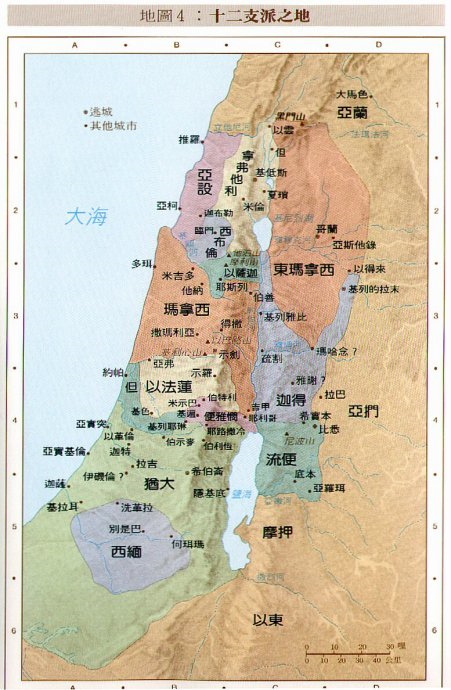
\includegraphics[width=6in]{BLiShiFigs/taocheng}
	 \caption{逃城}
	 \label{fig:2} 
	 \end{center}
	 \end{figure}

\subsubsection{逃城目的 20:1-6}
耶和華曉諭約書亞說： 2 「你吩咐以色列人說：你們要照著我藉摩西所曉諭你們的，為自己設立逃城， 3 使那無心而誤殺人的可以逃到那裡。這些城可以做你們逃避報血仇人的地方。 4 那殺人的要逃到這些城中的一座城，站在城門口，將他的事情說給城內的長老們聽。他們就把他收進城裡，給他地方，使他住在他們中間。 5 若是報血仇的追了他來，長老不可將他交在報血仇的手裡，因為他是素無仇恨，無心殺了人的。 6 他要住在那城裡，站在會眾面前聽審判，等到那時的大祭司死了，殺人的才可以回到本城本家，就是他所逃出來的那城。」

\subsubsection{逃城地点 20:7-9}
\begin{wraptable}{r}{9cm}
\centering
\vspace{-1.cm}
\begin{tabular}{|c|c||c|c|}\hline\hline
 \multicolumn{2}{|m{5cm}||}{\centering 河西} & \multicolumn{2}{m{2.5cm}|}{\centering 河東} \\\hline
 拿弗他利 &基低斯&流便&比悉    \\\hline
 以法蓮山地&示劍& 迦得&拉末  \\\hline
 猶大山地&基列亞巴(希伯崙)&瑪拿西&哥蘭 \\\hline
\end{tabular}
\caption{逃城}
\end{wraptable}
於是，以色列人在拿弗他利山地分定加利利的基低斯，在以法蓮山地分定示劍，在猶大山地分定基列亞巴，基列亞巴就是希伯崙。又在約旦河外耶利哥東，從魯本支派中，在曠野的平原設立比悉，從迦得支派中設立基列的拉末，從瑪拿西支派中設立巴珊的哥蘭。這都是為以色列眾人和在他們中間寄居的外人所分定的地邑，使誤殺人的都可以逃到那裡，不死在報血仇人的手中，等他站在會眾面前聽審判。


   

\subsubsection{利未人求城邑 21:1-3}
那時，利未人的眾族長來到祭司以利亞撒和嫩的兒子約書亞並以色列各支派的族長面前， 2 在迦南地的示羅對他們說：「從前耶和華藉著摩西吩咐給我們城邑居住，並城邑的郊野可以牧養我們的牲畜。」 3 於是以色列人照耶和華所吩咐的，從自己的地業中，將以下所記的城邑和城邑的郊野給了利未人。

\subsubsection{哥轄族的城邑 21:4-5}
\begin{table}[H]
\centering
\begin{tabular}{|c|c|c|}
\hline
\hline
 猶大& 西緬& 便雅憫\\\hline
 \textbf{基列亞巴},立拿,雅提珥,以實提莫,何崙,底璧,淤他,伯示麥& 亞因& 基遍,迦巴,亞拿突,亞勒們\\\hline
\end{tabular}
\caption{亞倫的子孫(13座城)}
\end{table}
為哥轄族拈鬮，利未人的祭司，亞倫的子孫，從猶大支派、西緬支派、便雅憫支派的地業中，按鬮得了十三座城。

5 哥轄其餘的子孫，從以法蓮支派、但支派、瑪拿西半支派的地業中，按鬮得了十座城。

\begin{table}[H]
\centering
\begin{tabular}{|c|c|c|}
\hline
\hline
 以法蓮&但&瑪拿西 \\\hline
 \textbf{示劍},基色,基伯先,伯和崙& 伊利提基,基比頓,亞雅崙,迦特臨門,& 他納,迦特臨門\\\hline
\end{tabular}
\caption{哥轄其餘的子孫(10座城)}
\end{table}

\subsubsection{革順的城邑 21:6}
\begin{table}[H]
\centering
\begin{tabular}{|c|c|c|c|}
\hline
\hline
 以薩迦&亞設&拿弗他利&瑪拿西\\\hline
基善,大比拉,耶末,隱干寧&米沙勒,押頓,黑甲,利合  &\textbf{基低斯},哈末多珥,加珥坦  & \textbf{哥蘭},比施提拉\\\hline
\end{tabular}
\caption{革順的子孫(13座城)}
\end{table}
哥轄其餘的子孫，從以法蓮支派、但支派、瑪拿西半支派的地業中，按鬮得了十座城。

\subsubsection{米拉利的城邑 21:7}
\begin{table}[H]
\centering
\begin{tabular}{|c|c|c|}
\hline
\hline
 流便&迦得&西布倫\\\hline
 \textbf{比悉},雅雜,基底莫,米法押 &\textbf{拉末},瑪哈念,希實本,雅謝  & 約念,加珥他,丁拿,拿哈拉 \\\hline
\end{tabular}
\caption{米拉利的子孫(12座城)}
\end{table}

\subsubsection{亞倫子孫做祭司的城邑十三座 21:8-19}
以色列人照著耶和華藉摩西所吩咐的，將這些城邑和城邑的郊野，按鬮分給利未人。 9  10 從猶大支派、西緬支派的地業中，將以下所記的城給了利未支派哥轄宗族亞倫的子孫，因為給他們拈出頭一鬮。 11 將猶大山地的基列亞巴和四圍的郊野給了他們（亞巴是亞衲族的始祖，基列亞巴就是希伯崙）， 12 唯將屬城的田地和村莊給了耶孚尼的兒子迦勒為業。 13 以色列人將希伯崙，就是誤殺人的逃城和屬城的郊野，給了祭司亞倫的子孫，又給他們立拿和屬城的郊野， 14 雅提珥和屬城的郊野，以實提莫和屬城的郊野， 15 何崙和屬城的郊野，底璧\footnote{約書亞記 15:14-17迦勒...又從那裡上去，攻擊底璧的居民，這底璧從前名叫基列西弗。迦勒說：「誰能攻打基列西弗將城奪取，我就把我女兒押撒給他為妻。」迦勒兄弟基納斯的兒子俄陀聶奪取了那城，迦勒就把女兒押撒給他為妻。}和屬城的郊野，亞因和屬城的郊野，淤他和屬城的郊野，伯示麥和屬城的郊野，共九座城，都是從這二支派中分出來的。 17 又從便雅憫支派的地業中給了他們基遍和屬城的郊野，迦巴和屬城的郊野， 18 亞拿突和屬城的郊野，亞勒們和屬城的郊野，共四座城。 19 亞倫子孫做祭司的共有十三座城，還有屬城的郊野。

\subsubsection{哥轄其餘的子孫城邑十座 21:20-26}
利未支派中哥轄的宗族，就是哥轄其餘的子孫，拈鬮所得的城有從以法蓮支派中分出來的。 21 以色列人將以法蓮山地的示劍，就是誤殺人的逃城和屬城的郊野，給了他們，又給他們基色和屬城的郊野， 22 基伯先和屬城的郊野，伯和崙和屬城的郊野，共四座城。 23 又從但支派的地業中給了他們伊利提基和屬城的郊野，基比頓和屬城的郊野， 24 亞雅崙和屬城的郊野，迦特臨門和屬城的郊野，共四座城。 25 又從瑪拿西半支派的地業中給了他們他納和屬城的郊野，迦特臨門和屬城的郊野，共兩座城。 26 哥轄其餘的子孫共有十座城，還有屬城的郊野。

\subsubsection{革順的城邑十三座 21:27-33}
以色列人又從瑪拿西半支派的地業中將巴珊的哥蘭，就是誤殺人的逃城和屬城的郊野，給了利未支派革順的子孫，又給他們比施提拉和屬城的郊野，共兩座城。 28 又從以薩迦支派的地業中給了他們基善和屬城的郊野，大比拉和屬城的郊野， 29 耶末和屬城的郊野，隱干寧和屬城的郊野，共四座城。 30 又從亞設支派的地業中給了他們米沙勒和屬城的郊野，押頓和屬城的郊野， 31 黑甲和屬城的郊野，利合和屬城的郊野，共四座城。 32 又從拿弗他利支派的地業中將加利利的基低斯，就是誤殺人的逃城和屬城的郊野，給了他們，又給他們哈末多珥和屬城的郊野，加珥坦和屬城的郊野，共三座城。 33 革順人按著宗族所得的城，共十三座，還有屬城的郊野。

\subsubsection{米拉利的城邑十二座 21:34-40}
其餘利未支派米拉利子孫，從西布倫支派的地業中所得的，就是約念和屬城的郊野，加珥他和屬城的郊野， 35 丁拿和屬城的郊野，拿哈拉和屬城的郊野，共四座城。 36 又從魯本支派的地業中給了他們比悉和屬城的郊野，雅雜和屬城的郊野， 37 基底莫和屬城的郊野，米法押和屬城的郊野，共四座城。 38 又從迦得支派的地業中，將基列的拉末，就是誤殺人的逃城和屬城的郊野，給了他們，又給他們瑪哈念和屬城的郊野， 39 希實本和屬城的郊野，雅謝和屬城的郊野，共四座城。 40 其餘利未支派的人，就是米拉利的子孫，按著宗族拈鬮所得的，共十二座城。

\subsubsection{耶和華應許賜福以色列應驗 21:41-45}
利未人在以色列人的地業中所得的城，共四十八座，並有屬城的郊野。 42 這些城四圍都有屬城的郊野，城城都是如此。

43 這樣，耶和華將從前向他們列祖起誓所應許的全地賜給以色列人，他們就得了為業，住在其中。 44 耶和華照著向他們列祖起誓所應許的一切話，使他們四境平安。他們一切仇敵中，沒有一人在他們面前站立得住。耶和華把一切仇敵都交在他們手中。 45 耶和華應許賜福給以色列家的話一句也沒有落空，都應驗了。



\section{約書亞最后的服事 22-24}

\subsection{打發兩個半支派的人回去 22:1-9}
當時，約書亞召了魯本人、迦得人和瑪拿西半支派的人來， 2 對他們說：「耶和華僕人摩西所吩咐你們的，你們都遵守了；我所吩咐你們的，你們也都聽從了。 3 你們這許多日子，總沒有撇離你們的弟兄，直到今日，並守了耶和華你們神所吩咐你們當守的。 4 如今耶和華你們神照著他所應許的，使你們弟兄得享平安，現在可以轉回你們的帳篷，到耶和華的僕人摩西在約旦河東所賜你們為業之地。 5 只要切切地謹慎遵行耶和華僕人摩西所吩咐你們的誡命、律法，愛耶和華你們的神，行他一切的道，守他的誡命，專靠他，盡心、盡性侍奉他。」 6 於是約書亞為他們祝福，打發他們去。他們就回自己的帳篷去了。
瑪拿西那半支派，摩西早已在巴珊分給他們地業。這半支派，約書亞在約旦河西，在他們弟兄中，分給他們地業。約書亞打發他們回帳篷的時候為他們祝福， 8 對他們說：「你們帶許多財物、許多牲畜和金、銀、銅、鐵，並許多衣服，回你們的帳篷去，要將你們從仇敵奪來的物與你們眾弟兄同分。」 9 於是魯本人、迦得人、瑪拿西半支派的人從迦南地的示羅起行，離開以色列人，回往他們得為業的基列地，就是照耶和華藉摩西所吩咐的得了為業之地。

\subsection{二支派半人築壇於約旦河濱 22:10}

流便人、迦得人和瑪拿西半支派的人到了靠近約旦河的一帶迦南地，就在約旦河那裡築了一座壇，那壇看著高大。 

\subsection{以色列人打發非尼哈見二支派半人 22:11-20}
\begin{table}[H]
\centering
\begin{tabular}{p{2.5cm}|p{2.95cm}|p{11.5cm}}\hline\hline
全會眾聚集&差派首领&見二支派半人会谈\\\hline
以色列人聽說流便人、迦得人、瑪拿西半支派的人靠近約旦河邊，在迦南地屬以色列人的那邊築了一座壇。全會眾一聽見，就聚集在示羅，要上去攻打他們。
&以色列人打發祭司以利亞撒的兒子非尼哈，往基列地去見流便人、迦得人、瑪拿西半支派的人，又打發十個首領與非尼哈同去，就是以色列每支派的一個首領，都是以色列軍中的統領。
&他們到了基列地，見流便人、迦得人和瑪拿西半支派的人，對他們說：「耶和華全會眾這樣說：你們今日轉去不跟從耶和華，干犯以色列的神，為自己築一座壇，悖逆了耶和華，這犯的是什麼罪呢？從前拜毗珥的罪孽還算小嗎？雖然瘟疫臨到耶和華的會眾，到今日我們還沒有洗淨這罪。你們今日竟轉去不跟從耶和華嗎？你們今日既悖逆耶和華，明日他必向以色列全會眾發怒。你們所得為業之地，若嫌不潔淨，就可以過到耶和華之地，就是耶和華的帳幕所住之地，在我們中間得地業。只是不可悖逆耶和華，也不可得罪我們，在耶和華我們神的壇以外為自己築壇。從前謝拉的曾孫亞干，豈不是在那當滅的物上犯了罪，就有憤怒臨到以色列全會眾嗎？那人在所犯的罪中不獨一人死亡。」\\\hline
 \end{tabular}
\caption{以色列人打發非尼哈見二支派半人}
\end{table}





\subsection{二支派半人解釋原因 22:21-29}
\begin{table}[H]
\centering
\begin{tabular}{p{4.75cm}|p{4.cm}|p{8.25cm}}\hline\hline
向神祷告&惧怕原因&築壇目的-做證據\\\hline
於是流便人、迦得人、瑪拿西半支派的人回答以色列軍中的統領說：「大能者神耶和華！大能者神耶和華！他是知道的，以色列人也必知道。我們若有悖逆的意思，或是干犯耶和華——願你今日不保佑我們——為自己築壇，要轉去不跟從耶和華，或是要將燔祭、素祭、平安祭獻在壇上，願耶和華親自討我們的罪。
&我們行這事並非無故，是特意做的，說恐怕日後你們的子孫對我們的子孫說：『你們與耶和華以色列的神有何關涉呢？因為耶和華把約旦河定為我們和你們這流便人、迦得人的交界。你們與耶和華無份了！』這樣，你們的子孫就使我們的子孫不再敬畏耶和華了。
&因此我們說，不如為自己築一座壇，不是為獻燔祭，也不是為獻別的祭，乃是為你我中間和你我後人中間做證據，好叫我們也在耶和華面前獻燔祭、平安祭和別的祭侍奉他，免得你們的子孫日後對我們的子孫說：『你們與耶和華無份了！』所以我們說，日後你們對我們或對我們的後人這樣說，我們就可以回答說：『你們看我們列祖所築的壇是耶和華壇的樣式，這並不是為獻燔祭，也不是為獻別的祭，乃是為做你我中間的證據。』我們在耶和華我們神帳幕前的壇以外，另築一座壇，為獻燔祭、素祭和別的祭，悖逆耶和華，今日轉去不跟從他，我們斷沒有這個意思！」\\\hline
 \end{tabular}
\caption{築證壇原因}
\end{table}

\subsection{重修和睦二支派半人給壇起名叫證壇 22:30-34}
\begin{table}[H]
\centering
\begin{tabular}{p{8.cm}|p{6.2cm}|p{2.5cm}}\hline\hline
非尼哈對流便人、迦得人、瑪拿西人說&非尼哈回報以色列人&給壇起名證壇\\\hline
祭司非尼哈與會中的首領，就是與他同來以色列軍中的統領，聽見流便人、迦得人、瑪拿西人所說的話，就都以為美。祭司以利亞撒的兒子非尼哈對流便人、迦得人、瑪拿西人說：「今日我們知道耶和華在我們中間，因為你們沒有向他犯了這罪。現在你們救以色列人脫離耶和華的手了！」&
 祭司以利亞撒的兒子非尼哈與眾首領離了流便人、迦得人，從基列地回往迦南地，到了以色列人那裡，便將這事回報他們。以色列人以這事為美，就稱頌神，不再提上去攻打流便人、迦得人，毀壞他們所住的地了。
&流便人、迦得人給壇起名叫證壇，意思說：「這壇在我們中間證明耶和華是神。」\\\hline
 \end{tabular}
\caption{重修和睦二支派半人給壇起名叫證壇}
\end{table}




\subsection{約書亞最後的遺言 23-24}
\subsubsection{約書亞第一次招聚百姓 23:1-16}
\begin{table}[H]
\centering
\begin{tabular}{p{5.cm}|p{7.75cm}|p{4.25cm}}\hline\hline
神所應許&勸民侍奉耶和華&賜福禍患都必應驗\\\hline
\multirow{4}{5.cm}{耶和華使以色列人安靜，不與四圍的一切仇敵爭戰，已經多日。約書亞年紀老邁，就把以色列眾人的長老、族長、審判官並官長都召了來，對他們說：「我年紀已經老邁。耶和華你們的神因你們的緣故向那些國所行的一切事，你們親眼看見了，因那為你們爭戰的是耶和華你們的神。我所剪除和所剩下的各國，從約旦河起到日落之處的大海，我已經拈鬮分給你們各支派為業。耶和華你們的神必將他們從你們面前趕出去，使他們離開你們，你們就必得他們的地為業，正如耶和華你們的神所應許的。}
&所以，你們要大大壯膽，謹守遵行寫在摩西律法書上的一切話，
&\multirow{4}{4.25cm}{我現在要走世人必走的路。你們是一心一意地知道，耶和華你們神所應許賜福於你們的話沒有一句落空，都應驗在你們身上了。耶和華你們神所應許的一切福氣怎樣臨到你們身上，耶和華也必照樣使各樣禍患臨到你們身上，直到把你們從耶和華你們神所賜的這美地上除滅。你們若違背耶和華你們神吩咐你們所守的約，去侍奉別神，叩拜他，耶和華的怒氣必向你們發作，使你們在他所賜的美地上速速滅亡。}\\\cline{2-2}
&不可偏離左右。不可與你們中間所剩下的這些國民摻雜。他們的神，你們不可提他的名，不可指著他起誓，也不可侍奉、叩拜。&\\\cline{2-2}
&只要照著你們到今日所行的，專靠耶和華你們的神。因為耶和華已經把又大又強的國民從你們面前趕出，直到今日，沒有一人在你們面前站立得住。你們一人必追趕千人，因耶和華你們的神照他所應許的，為你們爭戰。你們要分外謹慎，愛耶和華你們的神。&\\\cline{2-2}
&你們若稍微轉去，與你們中間所剩下的這些國民聯絡，彼此結親，互相往來，你們要確實知道：耶和華你們的神必不再將他們從你們眼前趕出，他們卻要成為你們的網羅、機檻，肋上的鞭、眼中的刺，直到你們在耶和華你們神所賜的這美地上滅亡。&\\\hline

 \end{tabular}
\caption{重修和睦二支派半人給壇起名叫證壇}
\end{table}



\subsubsection{二次在示劍招聚百姓述說神恩 24:1-13}
\begin{table}[H]
\centering
\begin{tabular}{p{4.5cm}|p{4.cm}|p{3.5cm}|p{4.5cm}}\hline\hline
祖宗亞伯拉罕蒙召&領以色列出埃及过曠野&得約旦河東之地&得約旦河西之地\\\hline
約書亞將以色列的眾支派聚集在示劍，召了以色列的長老、族長、審判官並官長來。他們就站在神面前，約書亞對眾民說：「耶和華以色列的神如此說：『古時你們的列祖，就是亞伯拉罕和拿鶴的父親他拉，住在大河那邊侍奉別神，我將你們的祖宗亞伯拉罕從大河那邊帶來，領他走遍迦南全地，又使他的子孫眾多，把以撒賜給他。又把雅各和以掃賜給以撒，將西珥山賜給以掃為業。 &
 後來雅各和他的子孫下到埃及去了。我差遣摩西、亞倫，並照我在埃及中所行的降災於埃及，然後把你們領出來。我領你們列祖出埃及，他們就到了紅海，埃及人帶領車輛馬兵追趕你們列祖到紅海。你們列祖哀求耶和華，他就使你們和埃及人中間黑暗了，又使海水淹沒埃及人。我在埃及所行的事，你們親眼見過。你們在曠野也住了許多年日。
&我領你們到約旦河東亞摩利人所住之地，他們與你們爭戰，我將他們交在你們手中，你們便得了他們的地為業，我也在你們面前將他們滅絕。那時，摩押王西撥的兒子巴勒起來攻擊以色列人，打發人召了比珥的兒子巴蘭來咒詛你們。我不肯聽巴蘭的話，所以他倒為你們連連祝福。這樣，我便救你們脫離巴勒的手。
&你們過了約旦河，到了耶利哥。耶利哥人、亞摩利人、比利洗人、迦南人、赫人、革迦撒人、希未人、耶布斯人都與你們爭戰，我把他們交在你們手裡。 我打發黃蜂飛在你們前面，將亞摩利人的二王從你們面前攆出，並不是用你的刀，也不是用你的弓。我賜給你們地土，非你們所修治的；我賜給你們城邑，非你們所建造的。你們就住在其中，又得吃非你們所栽種的葡萄園，橄欖園的果子。』\\\hline
 \end{tabular}
\caption{二次在示劍招聚百姓述說神恩}
\end{table}


\subsubsection{勸民侍奉耶和華 24:14-15}
「現在你們要敬畏耶和華，誠心實意地侍奉他，將你們列祖在大河那邊和在埃及所侍奉的神除掉，去侍奉耶和華。若是你們以侍奉耶和華為不好，今日就可以選擇所要侍奉的，是你們列祖在大河那邊所侍奉的神呢，是你們所住這地的亞摩利人的神呢？至於我和我家，我們必定侍奉耶和華。」

\subsubsection{在示劍與民立約 24:16-28}
\begin{table}[H]
\centering
\begin{tabular}{p{7.75cm}|p{9.25cm}}\hline\hline
百姓&約書亞\\\hline
百姓回答說：「我們斷不敢離棄耶和華去侍奉別神！因耶和華我們的神曾將我們和我們列祖從埃及地的為奴之家領出來，在我們眼前行了那些大神蹟，在我們所行的道上、所經過的諸國，都保護了我們。耶和華又把住此地的亞摩利人都從我們面前趕出去。所以，我們必侍奉耶和華，因為他是我們的神。」&約書亞對百姓說：「你們不能侍奉耶和華！因為他是聖潔的神，是忌邪的神，必不赦免你們的過犯罪惡。你們若離棄耶和華去侍奉外邦神，耶和華在降福之後，必轉而降禍於你們，把你們滅絕。」\\\hline
百姓回答約書亞說：「不然，我們定要侍奉耶和華。」&約書亞對百姓說：「你們選定耶和華，要侍奉他，你們自己做見證吧！」\\\hline
他們說：「我們願意做見證！」&約書亞說：「你們現在要除掉你們中間的外邦神，專心歸向耶和華以色列的神。」 \\\hline
百姓回答約書亞說：「我們必侍奉耶和華我們的神，聽從他的話。」當日，約書亞就與百姓立約，在示劍為他們立定律例、典章。&約書亞將這些話都寫在神的律法書上，又將一塊大石頭立在橡樹下耶和華的聖所旁邊。 約書亞對百姓說：「看哪，這石頭可以向我們做見證，因為是聽見了耶和華所吩咐我們的一切話。倘或你們背棄你們的神，這石頭就可以向你們做見證。(「倘若」云云或作「所以要向你們做見證，免得你們背棄耶和華你們的神」)」於是約書亞打發百姓各歸自己的地業去了。\\\hline
 \end{tabular}
\caption{在示劍與民立約}
\end{table}

\subsubsection{約書亞逝世 24:29-33}
\begin{table}[H]
\centering
\begin{tabular}{p{8.75cm}|p{5.cm}|p{2.75cm}}\hline\hline
 約書亞&約瑟&以利亞撒 \\\hline
這些事以後，耶和華的僕人嫩的兒子約書亞，正一百一十歲，就死了。以色列人將他葬在他地業的境內，就是在以法蓮山地的亭拿西拉，在迦實山的北邊。約書亞在世和約書亞死後，那些知道耶和華為以色列人所行諸事的長老還在的時候，以色列人侍奉耶和華。&以色列人從埃及所帶來約瑟的骸骨，葬埋在示劍，就是在雅各從前用一百塊銀子向示劍的父親哈抹的子孫所買的那塊地裡，這就做了約瑟子孫的產業。&亞倫的兒子以利亞撒也死了，就把他葬在他兒子非尼哈以法蓮山地所得的小山上。\\\hline
\end{tabular}
\caption{約書亞逝世}
\end{table}











